In the last chapter, we have covered means to understand variability,
synthesize variability models for a given software system, and to select sample
sets of configurations. To enable the assessment of performance evolution for
configurable software systems, the next step in our methodology takes into
account the dimension of time. As software evolves, multiple versions, or
called revisions, of a software system exist. In this chapter, we address the
question of how we can assess performance for multiple versions. Moreover, we
ask whether we can describe a configurable software systems’ performance
evolution history without exhaustively assessing all versions by selecting only
a sample set of versions. As illustrated in the methodological road-map in
Figure~\ref{fig:roadmap_2}, we summarize these two questions with the task of
\emph{revision sampling}.

\begin{figure}[h!]
	\centering
	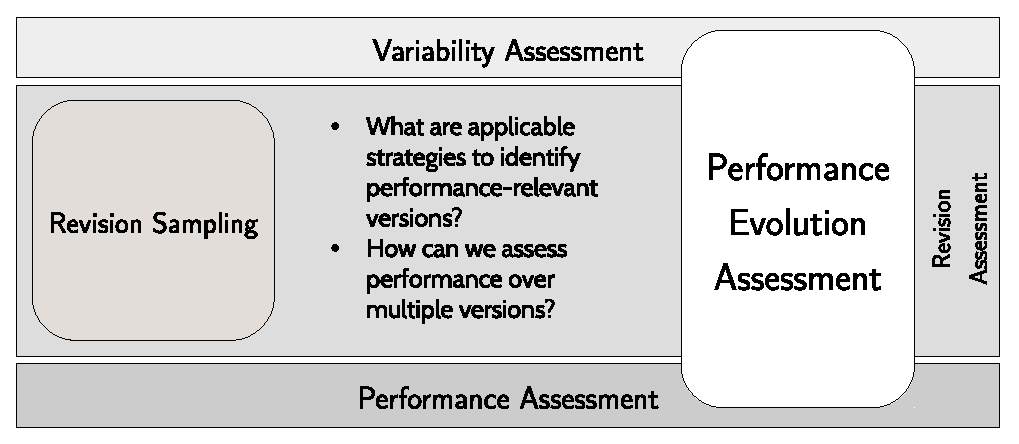
\includegraphics[width=0.99\textwidth]{images/process_revassesment.eps}
	\caption{Methodological road-map: questions to address with revision
	assessment.}
	\label{fig:roadmap_2}
\end{figure}

The chapter is organized as follows. In section~\ref{sec:towards_revsampling} we
present the methodological requirements for a designing and selecting a revision sampling
strategy. In section ~\ref{sec:revsampling_strat} we propose five approaches to
revision sampling. In
section~\ref{sec:revsampling_eval} we evaluate the different approaches against
exhaustive measurements of a selection of configurable software systems.
Finally, in section~\ref{sec:revsampling_method} we conclude the chapter and
discuss the approaches' applicability in the context of our methodology.

\section{Towards Revision Sampling}\label{sec:towards_revsampling}
Research so far has addressed the assessment of a software system’s revision
history under the umbrella of repository mining, for instance, to localize bugs
\citep{moin_bug_2010} or performance regression \citep{heger_automated_2013}.
Nonetheless, so far there exists little to no research addressing the question
what the choice of versions might reveal about performance evolution. The task
of selecting resources and a sample set of versions to analyze can be conceived
as a sampling strategy, where the objective is to cover interesting entities
(performance changes, in our case) while trying to limit the sample size to
keep the required effort reasonable. Before we present different approaches to
select a sample set of revisions, we define general cornerstones for
evaluating a sample set of revisions as well as respective revision sampling
strategies.

\paragraph{Revision Sample Set.} The first question is, what criteria we take as
a basis for rating a sample set of revisions as \emph{meaningful}. First, our intention
is to obtain a representative description of a software system’s performance
change history while only assessing a fraction of revisions. That is, assessing
a representative sample of revisions should yield a performance change history
similar to the assessment of all revisions. Since we are interested in
revisions for which performance measurements change, those revisions should be
contained in a representative sample. Second, especially in the context of
variability, a performance change might only affect a subset of the assessed
configurations. A representative sample set, therefore, should describe a
history of significant performance changes with respect to all variants
assessed. We consider a performance change to be significant, if it affects a
significant portion of the sample of variants (\emph{effect range}) and if the
relative change in performance measurements is significantly large (\emph{effect
magnitude}).

\begin{figure}[h!]
	\centering
	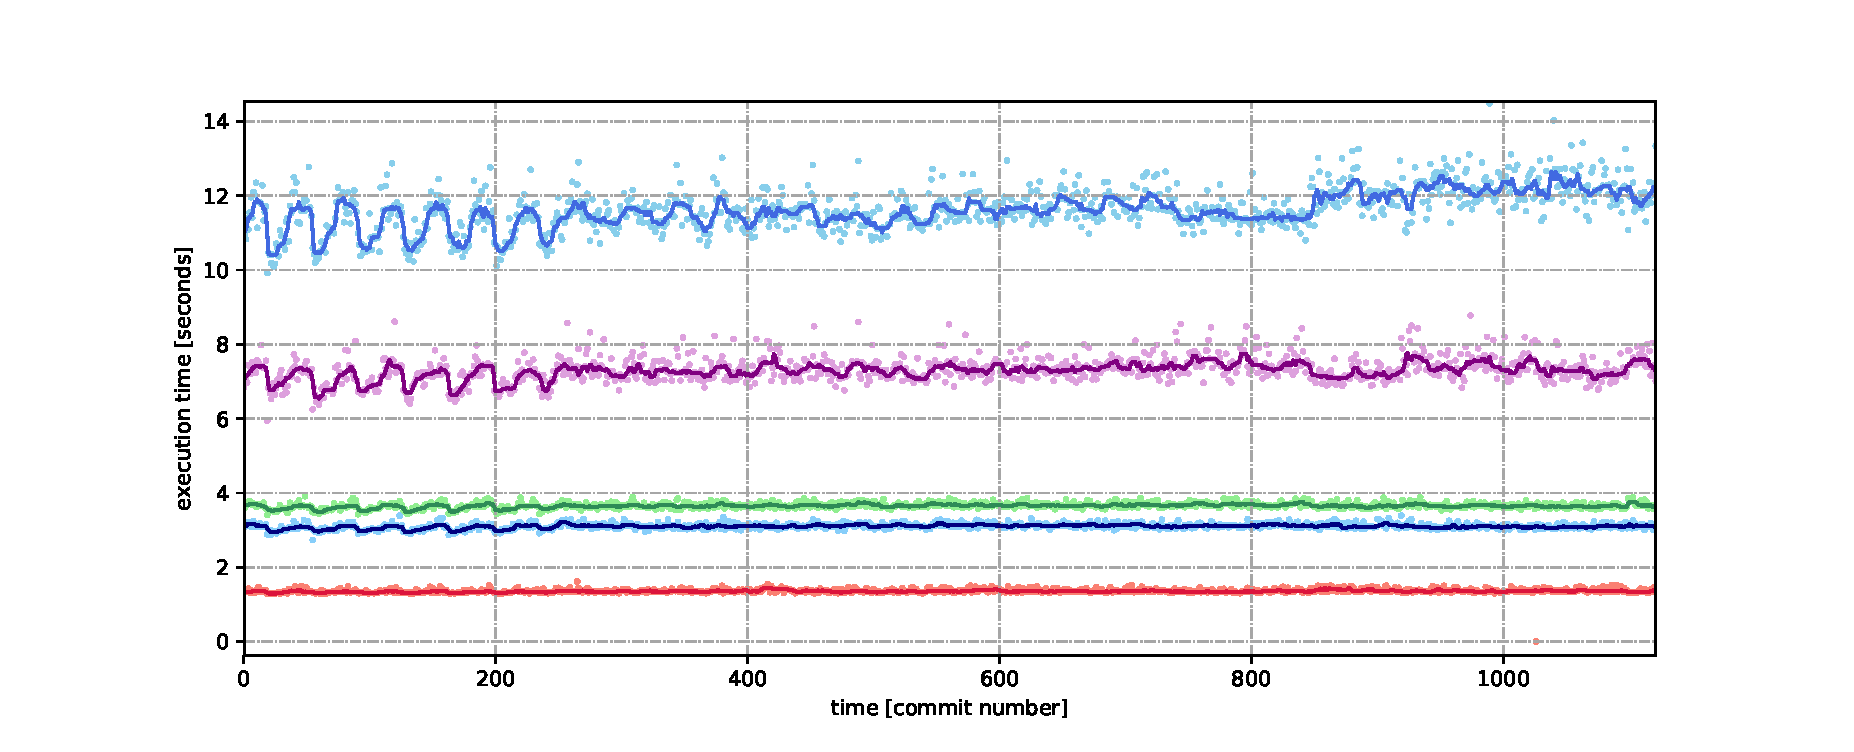
\includegraphics[width=0.99\textwidth]{images/xz_sample_evolution.eps}
	\caption{Performance history for GNU XZ: five different variants}
	\label{fig:xz_evosample}
\end{figure}

To illustrate the two facets of performance changes, in
Figure~\ref{fig:xz_evosample} we present a history of performance measurements
(execution time in this case) for a small-scale configurable software system,
file compression tool called \emph{GNU XZ Utils}. The graphic illustrates
execution time measures for executing a standard compression benchmark for $1,135$
different versions and covers a version history of about nine years. 

In this excerpt, we only show the execution time measures of five different
variants, i.e., each version was assessed with five different configurations.
Each performance measurement is depicted by a single marker. In addition, we
provide a plot of a moving mean, to identify trends. We see that each variant
has a certain performance level, and overall, the performance measurements
remain stable. While the blue and purple variant are generally more volatile,
for all variants, we see performance measurements oscillating during the first
250 versions. With regard to the two facets of significance mentioned earlier,
not all variants are affected similarly by this effect to the same degree.

While the former significance criterion can unambiguously defined by a threshold
number of variants, for the latter one one needs to define how to summarize
relative performance change among all variants. For instance, a performance
change may have a significant magnitude, if the average deviation of
performance measurements for all variants is greater than a specified threshold
value.

\paragraph{Revision Sampling Strategies.} The second question addresses the
rationale behind a revision sampling strategy. To obtain representative sample sets, sampling
strategies are intended to utilize knowledge about the volume to select
sample sets from. For instance, pair-wise sampling aims to cover most feature
interactions. Similarly, we demand for a meaningful revision sampling strategy
to exhibit a certain rationale or coverage criterion. If we conceive a sampling
strategy as a binary classificator that, in our case, decides whether in a
revision a performance change is likely, or performance measurements might have
changed compared to prior commits, we want  this classifier to be sensitive,
i.e., to have a preferably high true positive rate. That is, a sampling
strategy is meaningful if we learn which revision features most likely indicate
performance changes.\\

In conclusion, when designing a revision sampling strategy, we ask for a
plausible rationale or coverage criterion with respect to performance changes.
A resulting sample set of revisions, in addition, is representative, if the
contained revisions sketch performance changes. For the context of this
methodology, we remain with a clear definition of when performance changes are
significant. Based on these assumptions, in the next section we propose a
selection of five revision sampling approaches based on different observations.
 
\section{Revision Sampling Strategies}\label{sec:revsampling_strat}
As there are no established approaches to select sample sets of versions for
configurable software systems, especially with respect to performance
assessment, in the following five subsections, we propose five different
strategies to address this problem. Our proposals utilize different sources of
information regarding the software system studied, or are inspired by
approaches that have shown to be applicable in different contexts. An overview
and classification of the five proposals is presented in
Figure~\ref{fig:revsampling_overview}. 
Our approaches can be grouped into two categories. The first category incorporates
meta-data about a commit, including its lifetime (how long it has been the
latest commit), and the number of lines of code modified by it. For the first
category, sampling strategies intend to achieve high coverage of the overall
version lifetime, or modifications, respectively. The proposals listed in the
second category may as well take into account meta-data, yet for a
different purpose. The classification-based proposals' use meta-data along with
performance measurements to learn and predict the likelihood of a commit
introducing performance changes. The remaining approach, in the overview
referred to as performance history approximation, adapts the bisection approach
by \cite{heger_automated_2013} mentioned earlier. The approach continuously expands a sample
set until no performance-changing commits can be identified.

\begin{figure}[t]
\centering
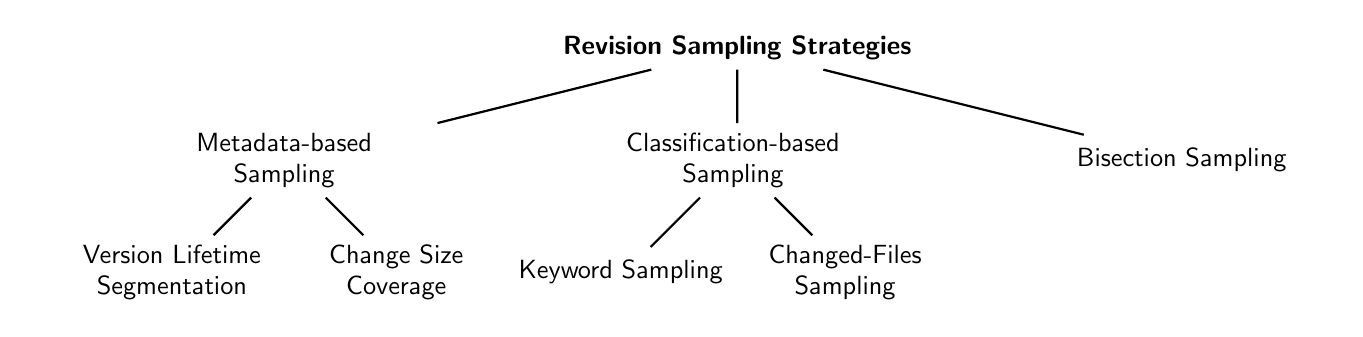
\begin{tikzpicture}[%sibling distance=15em,
level 1/.style={sibling distance=6cm},
level 2/.style={sibling distance=3cm}, 
level 3/.style={sibling distance=6cm},
  every node/.style = {rounded corners,
    draw, align=center,
    top color=white, bottom color=blue!20},thick,scale=0.95, every
    node/.style={scale=0.95}]
  \node {\sffamily\bfseries Revision Sampling Strategies}
    child { 
    	node [align=left] {
    		\begin{tabular}{c} 
    			{\sffamily \parbox{3.2cm}{\centering Metadata-based Sampling}}
    		\end{tabular}
    	}
    	child { 
    		node [align=left] {
    			\begin{tabular}{c} 
    				{\sffamily \parbox{3.2cm}{\centering Version Lifetime Segmentation}}
    			\end{tabular}
    		}
    	}
    	child { 
    		node [align=left] {
    			\begin{tabular}{c} 
    				{\sffamily \parbox{3.2cm}{\centering Change Size Coverage}}
    			\end{tabular}
    		}
    	} 
    }
    child { 
    	node [align=left] {
    		\begin{tabular}{c} 
    			{\sffamily \parbox{3.5cm}{\centering Classification-based Sampling}}
    		\end{tabular}
    	}
    	child { 
    		node [align=left] {
    			\begin{tabular}{c} 
    				{\sffamily \parbox{3.2cm}{\centering Keyword Sampling}}
    			\end{tabular}
    		}
    	}
    	child { 
    		node [align=left] {
    			\begin{tabular}{c} 
    				{\sffamily \parbox{3.2cm}{\centering Changed-Files Sampling}}
    			\end{tabular}
    		}
    	} 
    }
    child { 
    	node [align=left] {
    		\begin{tabular}{c} 
    			{\sffamily \parbox{3.2cm}{\centering Bisection Sampling}}
    		\end{tabular}
    	} 
    };
%    	child { 
%   		node [align=left] {
%	    		\begin{tabular}{c} 
%	    			{\sffamily \parbox{3cm}{\centering Hot-Spot Sampling}}
%	    		\end{tabular}
%    		}
%    	} 
%    };
\end{tikzpicture}

\caption{Overview of our proposed revision
sampling strategies.}\label{fig:revsampling_overview}
\end{figure}

\subsection{Keyword Sampling}
The first version sampling strategy we present is driven by the conception that
a commit message usually summarizes the changes of a commit in terms of what
has been implemented, modified, removed, or what problems have been fixed.
Commit messages can include keywords or phrases that indicate a performance
context, such as ``\textsf{fixed performance bug \ldots}'', or exhibit
information about the version of the software system, such as ``\textsf{bumped
version number to \ldots'}'.
Based on this information, we propose to use pattern matching to check whether a commit
message contains a keyword that might indicate a performance context, or a new
version, respectively. The sampling algorithm works as follows. Given a set of
keywords, such as ``\textsf{performance, bug, fix, slower, faster, \ldots}'', we
first derive the word stems for each keyword. Second, for each commit message, we split the
message into separate tokens and derive their corresponding word stems. Third,
we match all sets of resulting word stems (one set per commit message) against
the set of keyword sets and retain those commit messages, for which
sufficiently word stems are contained. As these commit messages contain our
previously defined keywords, we select the corresponding commits as our version
sample set.

This approach is simplistic and its accuracy clearly
depends on the quality of the initial selection of the keyword set as well as
the developer's discipline of documentation. Moreover, more sophisticated ways
to compute similarity between texts, such as the tf-idf-value and various
similarity metrics \citep{huang_similarity_2008}. However, we only propose this strategy to evaluate the overall applicability of approaches driven by text
similarity to the problem of version sampling.

\subsection{Version Lifetime Segmentation}
The second approach to select sample versions from the history of versions is
based on assumptions and observations obtained via repository mining. The
following approach is driven by the assumption that performance changes are
more likely to occur when the software system is revised frequently in a short
period of time. Not only is this simply due to a higher number of revisions. We
can also assume that if a software system has not been revised for a long
period of time, changes in terms of performance-relevant fixes were not
necessary, or have been deferred. Although postponing performance-relevant
fixes has become sort of a virtue \citep{molyneaux_art_2014}, for the latter
case there can exist other reasons, including organizational constraints, or
performance issues being undetected at that time. That is, we assume that those versions
that have been the latest version for a long time due to the absence of changes
as well as the necessity thereof can sketch a software systems performance
history. We do not assume that long-lasting versions introduce performance
changes, but they enable the segmentation of a software systems version history
in a way that it represents a large portion of the software systems lifetime.

\begin{figure}[!htb]
\def\tabularxcolumn#1{m{#1}}
\begin{tabularx}{\linewidth}{@{}cXX@{}}
\centering
\begin{tabular}{cc}
\subfloat[Activity graph for \texttt{GNU XZ}, generated from 1,135 versions
between December 8, 2007, and August 14, 2017.]
{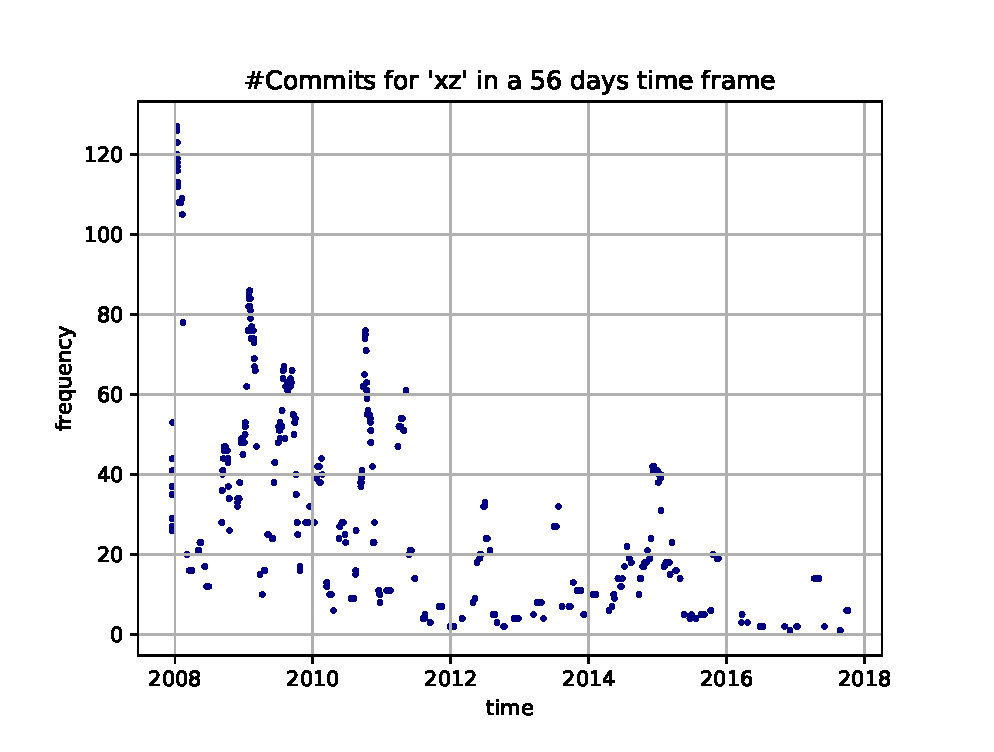
\includegraphics[width=0.48\textwidth]{images/activity_xz.eps}}
&
\subfloat[Activity graph for \texttt{x264}, generated from 2,851 versions
between June 3, 2004, and June 26,
2017.]{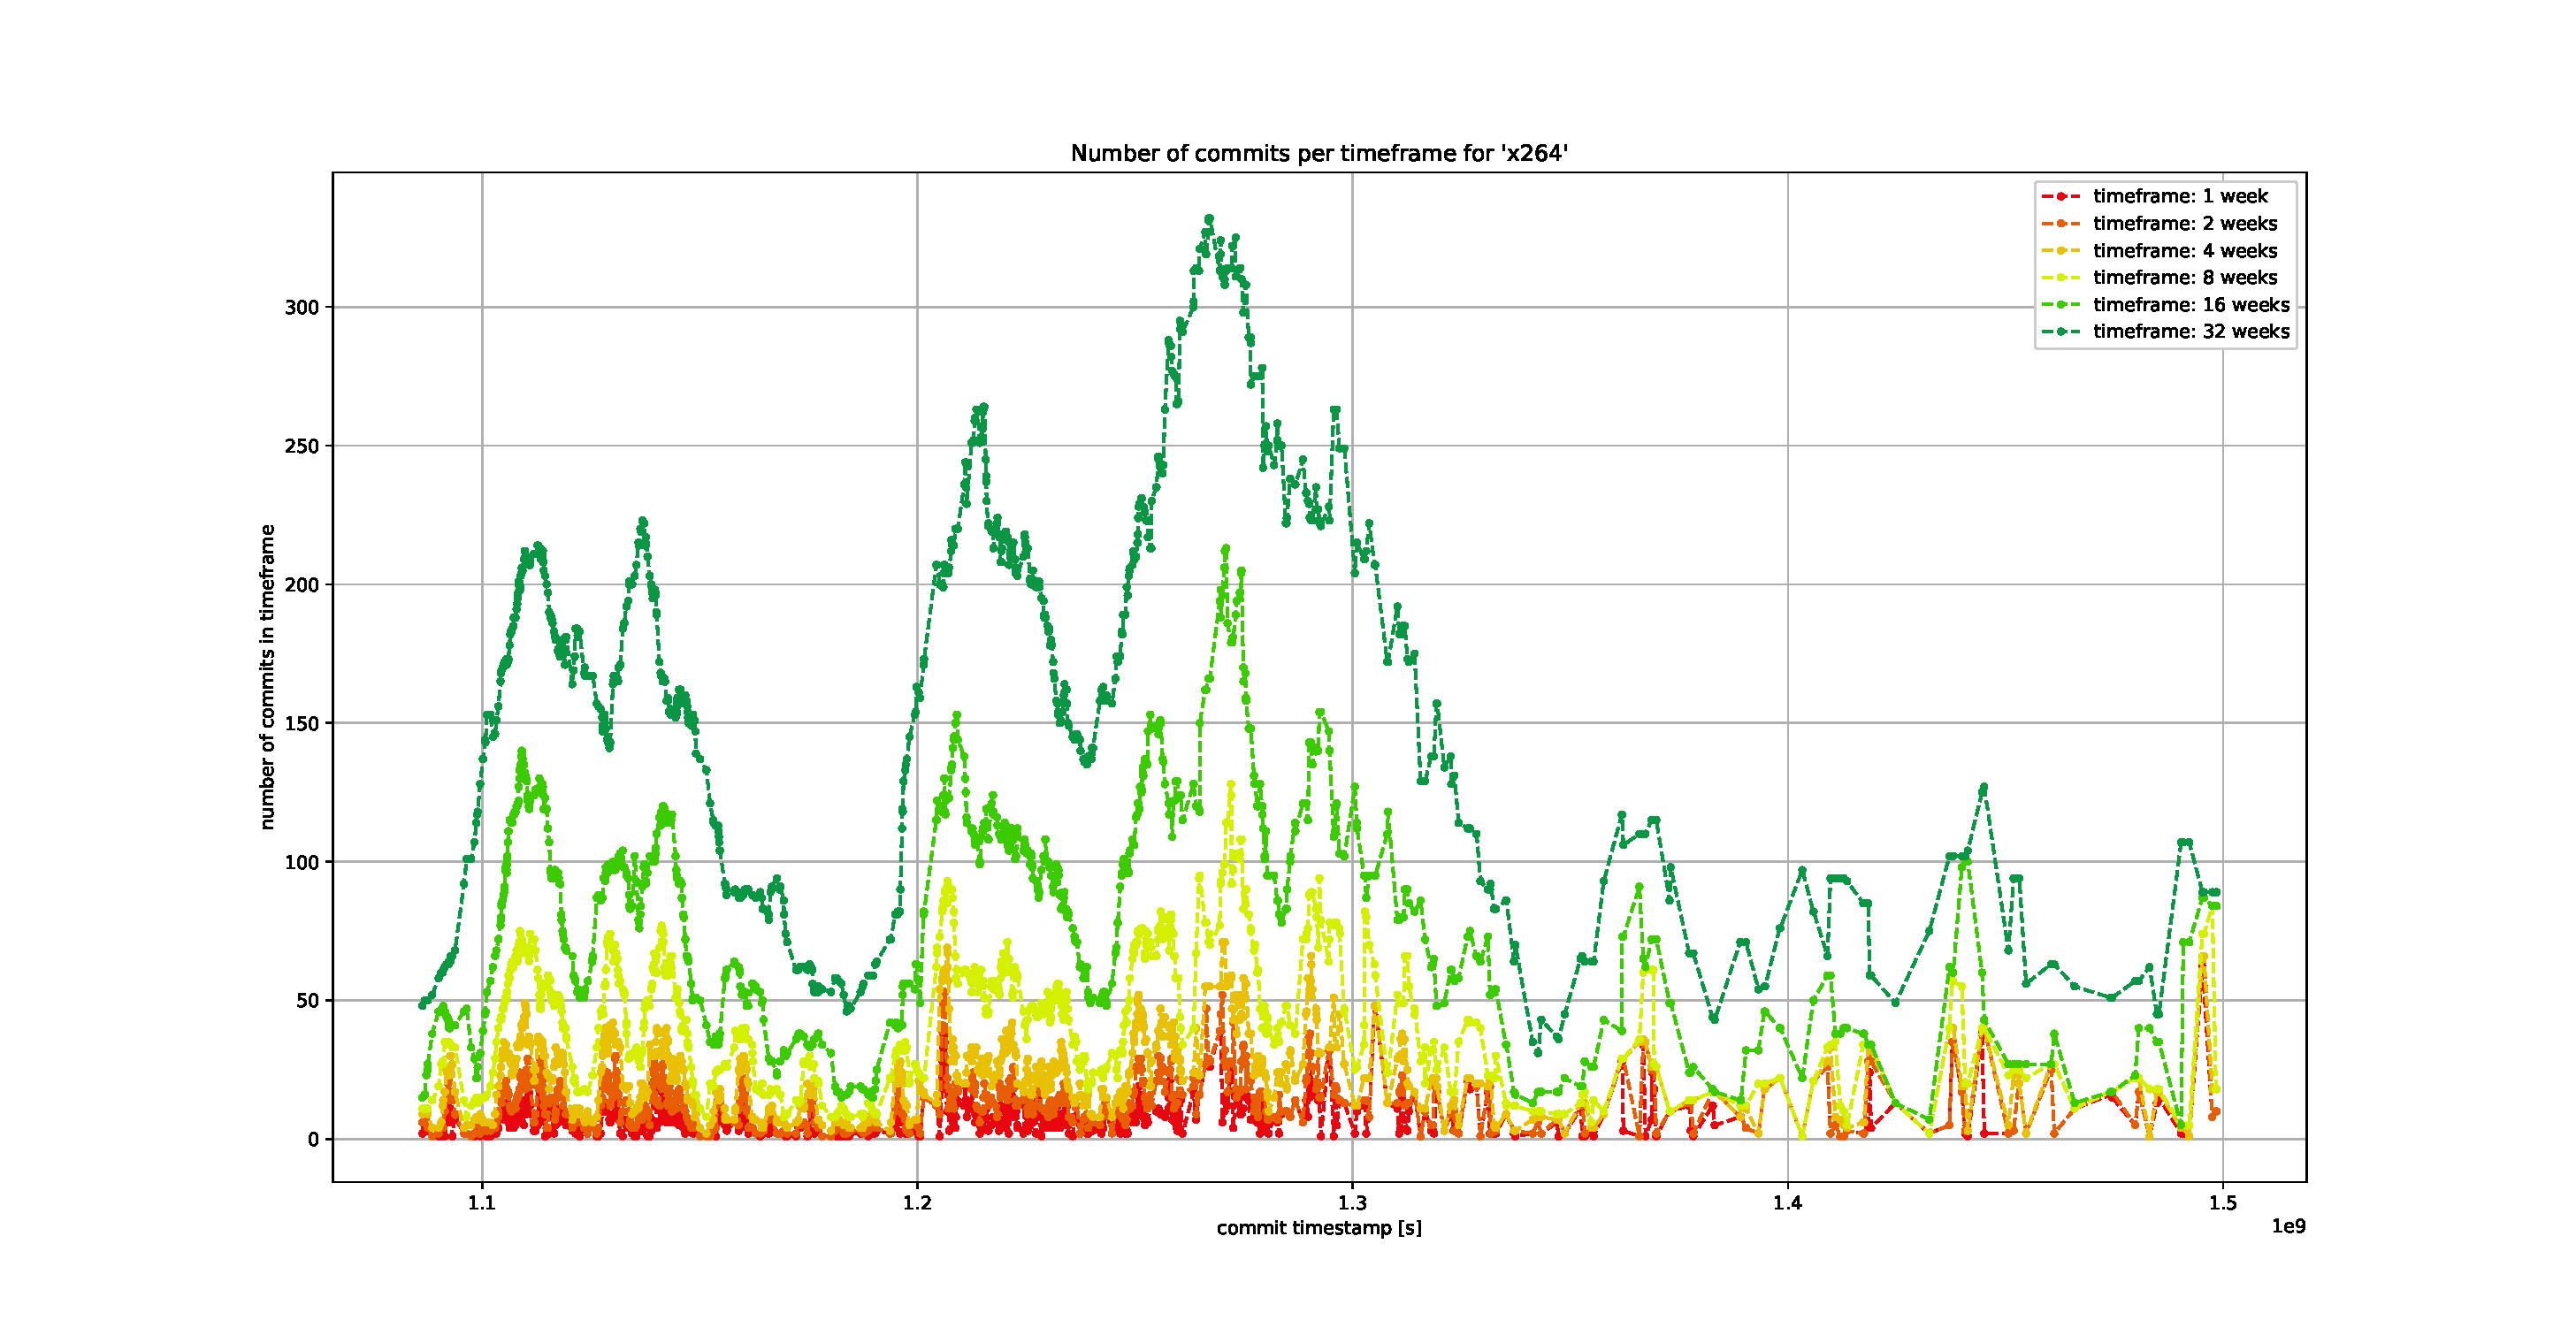
\includegraphics[width=0.48\textwidth]{images/activity_x264.eps}}\\
\end{tabular}
\end{tabularx}
\caption{Commit activity for two sample systems, the compression
utility \texttt{GNU XZ} and the video encoder \texttt{x264}. For each version,
the activity is measured as the number of commits that were pushed within a
certain time-frame of eight weeks.}
\label{fig:ActivityGraphs}
\end{figure}

Making the connection with our methodological context and the aim to design a
version sampling strategy, we intend to achieve a high “lifetime coverage” with
a small number of versions. For this reason, we have evaluated the “lifetime”
of versions of different software systems. In the following, lifetime of a
version or commit refers to the period of time between a commit and its
successor. We have investigated the distribution of version lifetime for two
open-source software systems, a free file compression tool, \emph{GNU XZ}, and a
free video encoder, \emph{x264}. – This selection is, by far, not
representative, yet the observations obtained from systems document our assumptions. Since we will
refer to those two and other systems for the evaluation, we answer how and why
these systems were selected in the evaluation in chapter\,\ref{chapter:6}.  –
The first observation regarding the lifetime of single versions is illustrated in
Figure~\ref{fig:ActivityGraphs} for the two software systems, respectively. The
figure, for each version, shows the activity during development of both systems.
For each commit, we have counted the number of commits preceding and succeeding
it within a four week time frame, respectively. One can see that for both
software systems we can identify spikes with a high commit frequency as well as
plunges with little to no commit activity. Moreover, if we look at the
histogram of all commits lifetime for both systems respectively as illustrated
in Figure~\ref{fig:version_lifetime}, we see that there actually are many
commits with a short lifetime (activity spikes) as well as only very few commits with a long lifetime (plunges).

\begin{figure}[!htb]
\def\tabularxcolumn#1{m{#1}}
\begin{tabularx}{\linewidth}{@{}cXX@{}}
\centering
\begin{tabular}{cc}
\subfloat[Distribution of time to next commits for \texttt{GNU XZ}]
{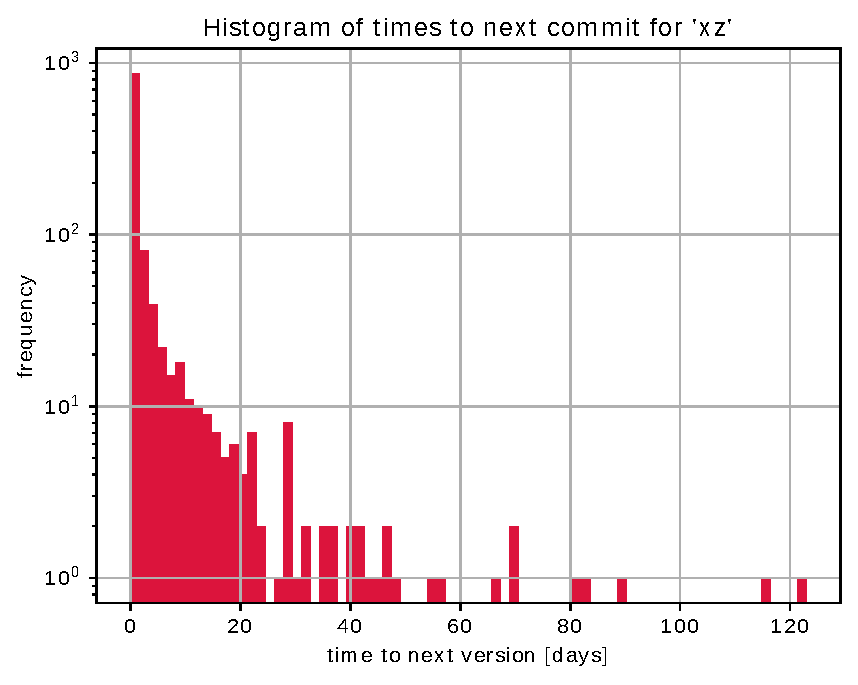
\includegraphics[width=0.48\textwidth]{images/commit_differences_xz.eps}}
&
\subfloat[Distribution of time to next commits for \texttt{x264}]
{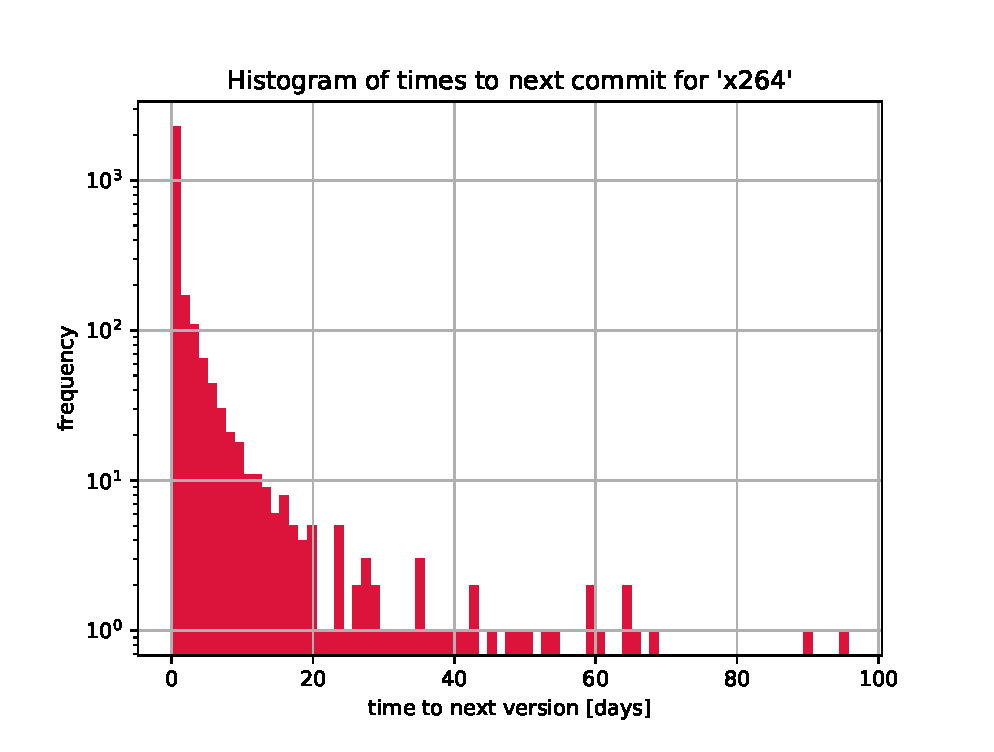
\includegraphics[width=0.48\textwidth]{images/commit_differences_x264.eps}}\\
\end{tabular}
\end{tabularx}
\caption{Distribution of time to next commits for two configurable software
systems, measured as the distance between a commit and its successor.}
\label{fig:version_lifetime}
\end{figure}

Based on the aforementioned assumptions as well as the distribution of version
lifetimes, when translating this in the context of a version sampling strategy,
we can achieve high ``lifetime coverage''  by selecting very few versions from a
list of versions sorted by lifetime in descending order. This sampling strategy
picks the longest-lasting commits until a desired coverage threshold, or
version count threshold number is reached. This sample selection of commits is a
segmentation or clustering of the overall version history. We assume that each
segment represents a (sort of) steady state of the software systems performance
history.

\subsection{Change Size Coverage}\label{sec:changesizesampling}
The third approach we propose adapts the idea of the previously mentioned
version lifetime segmentation. The following sampling strategy design is driven
by the assumption that a version or commit is more likely to introduce
performance changes to a software system if it modifies a large portion of
the code base. We assume that the effect of modifying a single line of code is
not as significant as modifying multiple lines of code. Of course, modifications can
accumulate, or trigger already existing interactions, yet from a black-box
perspective, commits affecting more lines of code are more likely to introduce
performance changes or to trigger interactions. That is, for designing a
version sampling strategy, we aim to cover most of all changes made to the
software system with a few number of versions. Similar to the assessment of
version lifetime in Figures~\ref{fig:ActivityGraphs} and
\ref{fig:version_lifetime}, we have investigated the distribution of commit
sizes in terms of lines of code for the two software systems \emph{GNU XZ} and
\emph{x264}. As illustrated in Figure~\ref{fig:version_size}, we see that, by far, most
commits modify less than 2,000 lines of code, whereas very few commits modify
or add larger code sections.

\begin{figure}[th!]
\def\tabularxcolumn#1{m{#1}}
\begin{tabularx}{\linewidth}{@{}cXX@{}}
\centering
\begin{tabular}{cc}
\subfloat[Distribution of changed lines per commit for \texttt{GNU XZ}]
{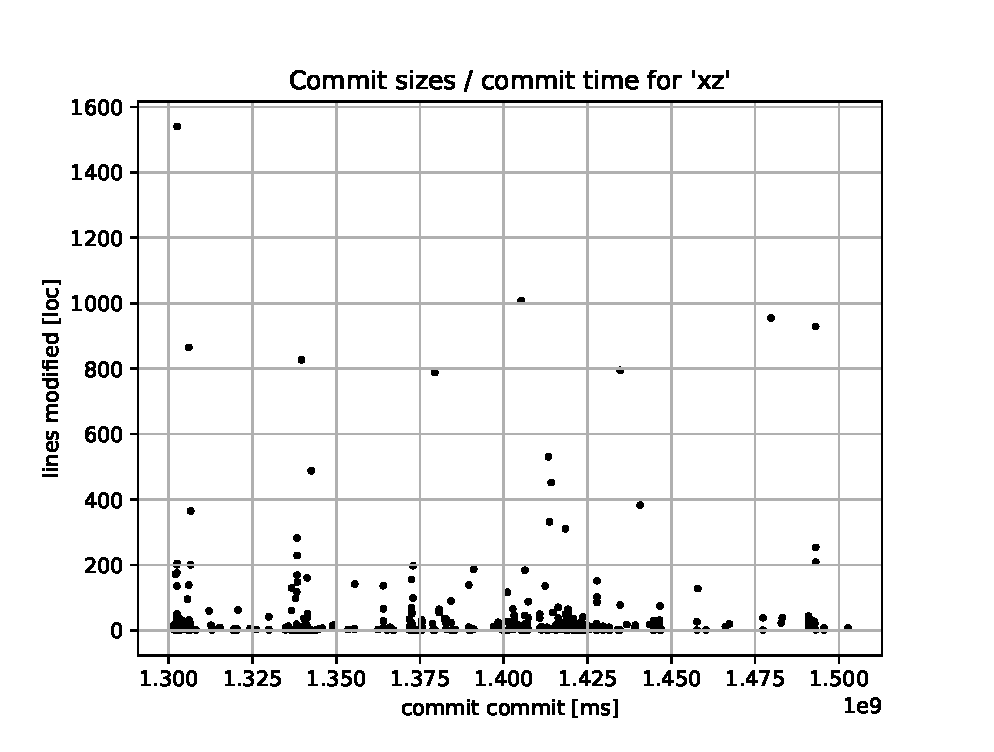
\includegraphics[width=0.48\textwidth]{images/commit_sizes_xz.eps}}
&
\subfloat[Distribution of changed lines per commit for
\texttt{x264}]{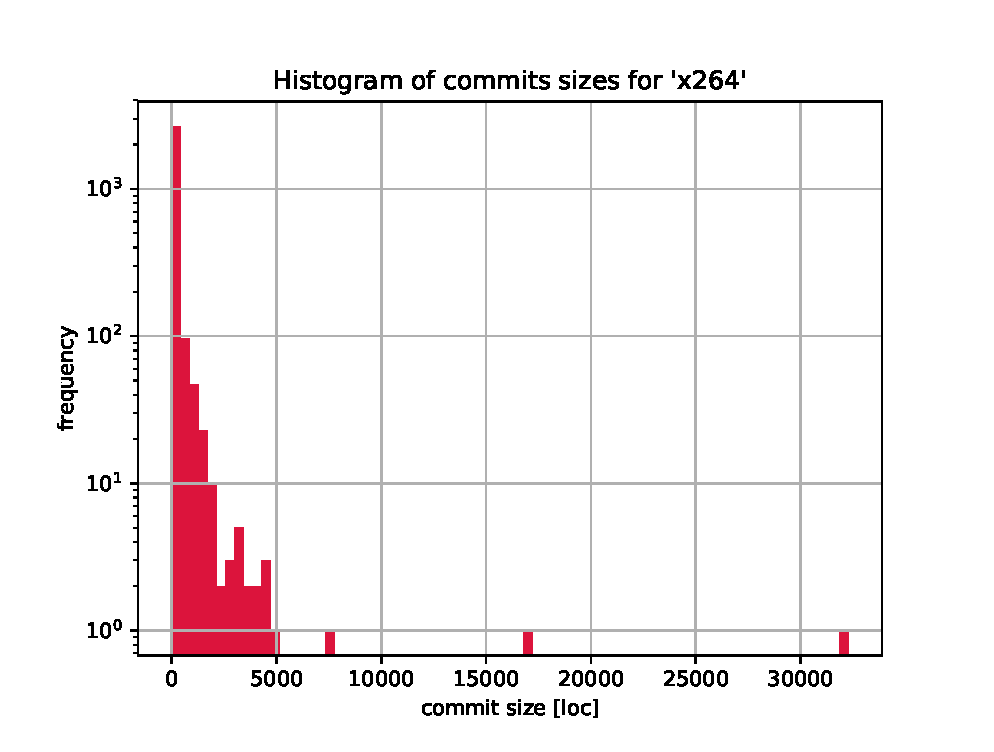
\includegraphics[width=0.48\textwidth]{images/commit_sizes_x264.eps}}\\
\end{tabular}
\end{tabularx}
\caption{Distribution of commit sizes in lines of code for two configurable
software systems, \texttt{GNU XZ} and \texttt{x264}.}
\label{fig:version_size}
\end{figure}

Based on these observations and given the assumption that larger commits are
more likely to introduce performance changes, we propose to obtain a sample of
versions by selecting versions from a list of versions sorted by commit size in
a descending order. Similarly to version lifetime segmentation, one can specify
a threshold of sample set size or commit size coverage to achieve. We assume
that a sample set of versions obtained using this approach is likely to cover
significant performance changes since a larger portion of the overall change
history is covered.

\subsection{Bisection Sampling}
The next sampling strategy that we propose is an adaption of the revision
sampling approach used by \cite{heger_automated_2013}. For a software system’s
 version history along with test cases and corresponding performance
 measurements, the
authors aim to identify those commits which may have introduced performance
regression. The authors have used a binary-search-like approach to continuously
bisect the version history to find commits for which performance measurements
deviate significantly from previously measured ones. Once a relevant commit is
identified, it can be subject of further root-cause analysis.

We adapt this approach to extract performance-relevant commits given an initial
sample of versions along with performance measurements. A performance-relevant
commit in this context is a commit for which performance measurements
significantly deviate from measurements of preceding commits. The sampling
strategy is applied as follows. 

\begin{wrapfigure}{R}{0.5\textwidth}
 \begin{center}
   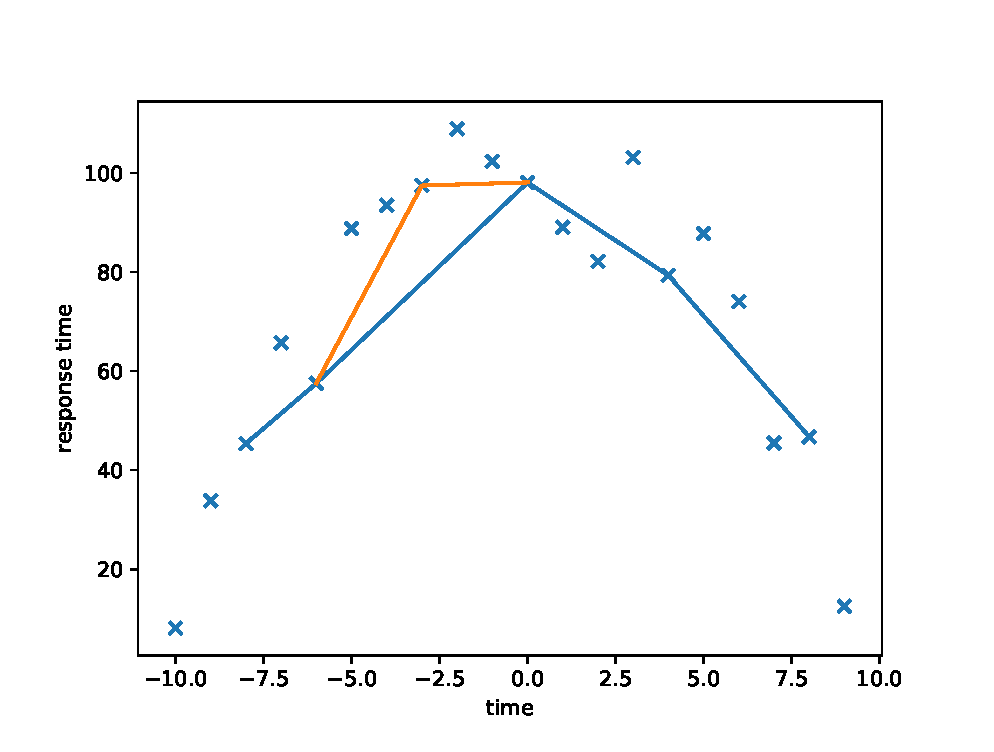
\includegraphics[width=0.5\textwidth]{images/inverse_douglas_peucker}
 \end{center}
\vspace{-5pt}
 \caption{Given a initial sample of five versions and four segments (blue
 line), the steepest segment is bisected and replaced by two segments
 (orange).
The first of the orange segments is steeper than the segment that was
bisected. \label{fig:example_bisection}}
\end{wrapfigure}

Given an initial sample of $n$ versions and
corresponding performance measurements, the version history is segmented into
$n-1$ segments. Each segment is clearly specified by two commits. For each
segment $s_i$, the algorithm computes the difference in performance
 measures $\delta_i$ for the start and the end commit. The segment with the
 largest deviation then is bisected. For the resulting two segments $\delta_{i_1}$ and $\delta_{i_2}$, the performance measurement differences are calculated. If the
absolute difference between $\delta_{i_1}$ and  $\delta_{i_2}$ is greater than
zero, one of the two children segments is ``steeper'', i.e., has a greater
performance measurement difference than the parent segment as exemplified in
Figure~\ref{fig:example_bisection}.

One can specify a minimum difference threshold to retain those resulting
segments. This procedure is repeated until no further segments can be bisected without violating the
minimum performance difference threshold. That is, the algorithm approximates
an interpolation of the overall performance history while focusing on sketching
the steepest changes. In addition to selecting an initial sample randomly, we
also propose to use version lifetime segmentation sampling to obtain
segmentation of the version history that segments it with respect to development
activity.

\subsection{Changed-Files Sampling}\label{sec:changedfiles}
The last version sampling strategy that we are going to present is a binary
classifier that predicts whether a commit is likely to introduce performance
changes. The idea behind this classifier is that performance changes might
depend on changes in specific code sections or combinations thereof. For each
commit we can retrieve which code sections, or files have been modified. If
there exists a relation between a commit’s file change set and performance
changes, we could learn it via machine learning and consequently predict
the performance change likelihood for arbitrary commits.

We propose a sampling strategy that is based on a initial training selection of
commits to learn a possible relation between a commit’s set of changed files
and performance changes. For each commit in the initial learning set, the
performance difference to its predecessor is calculated. Since we are
interested in any change in performance, not just performance degradation, we
consider the absolute performance difference as the performance change introduced by that
commit. Next, we are using classification and regression trees (CARTs) to
approximate a function that maps a commit’s set of changed files to its
absolute performance change. If the classificator is accurate enough, it can be
used to rank the commits that are most likely to introduce performance
changes. The sampling strategy can be configured with two parameters, $a$, the
size of the set to learn performance change likelihood from, and $b$, the
actual sample size to return. While the first $a$ parameter determines the
number of performance measurements required by this strategy, the second one,
$b$, determines how many top-ranked revisions are returned by the sampling
strategy, and therefore the actual sample size.

Moreover, for this strategy, we can modify the way to select a training sample.
The simplest solution is to randomly select $a$ commits and assess performance
for them and their predecessors. One could also select an initial learning
sample based on heuristics to increase its informative value. For instance,
since we intend to learn possible relations between a commits file change
footprint and performance changes, we could apply the commit change size
sampling strategy presented in section\,\ref{sec:changesizesampling} to possibly
increase the informative value of our training sample by covering a large
portion of the version history's overall change.

\section{Strategy Evaluation}\label{sec:revsampling_eval}
In this subsection, we evaluate and compare the revision sampling strategies
described above with respect to their accuracy to approximate the overall
performance history of a software system. First, we  describe how we measure
accuracy for a given revision sample; second, we present our corpus of systems
we assess performance evolution for, and finally, we present and discuss the
different sampling strategies’ results.

\subsection{Evaluation Setup}
An accurate approximation of an overall performance
history in our context is a selection of revisions along with its performance measures, which accurately
sketches the performance history obtained from assessing all versions. From an
accurate approximation one should be able to identify the same trends as from
the overall performance history. We measure the accuracy of a given revision
sample as follows. First, for the revision sample, we interpolate missing
performance measurements based on the measurements for our sample. Second, we
smooth the overall performance history, i.e., the performance measurements of
all revisions, using a moving mean in order to sketch overall performance
trends. Third, we compare our smoothed performance history and our interpolated
approximation using the Pearson correlation coefficient. The more similar
our approximated curve is to the overall performance history, the greater the
correlation coefficient is. 

\begin{figure}[h!]
	\centering
	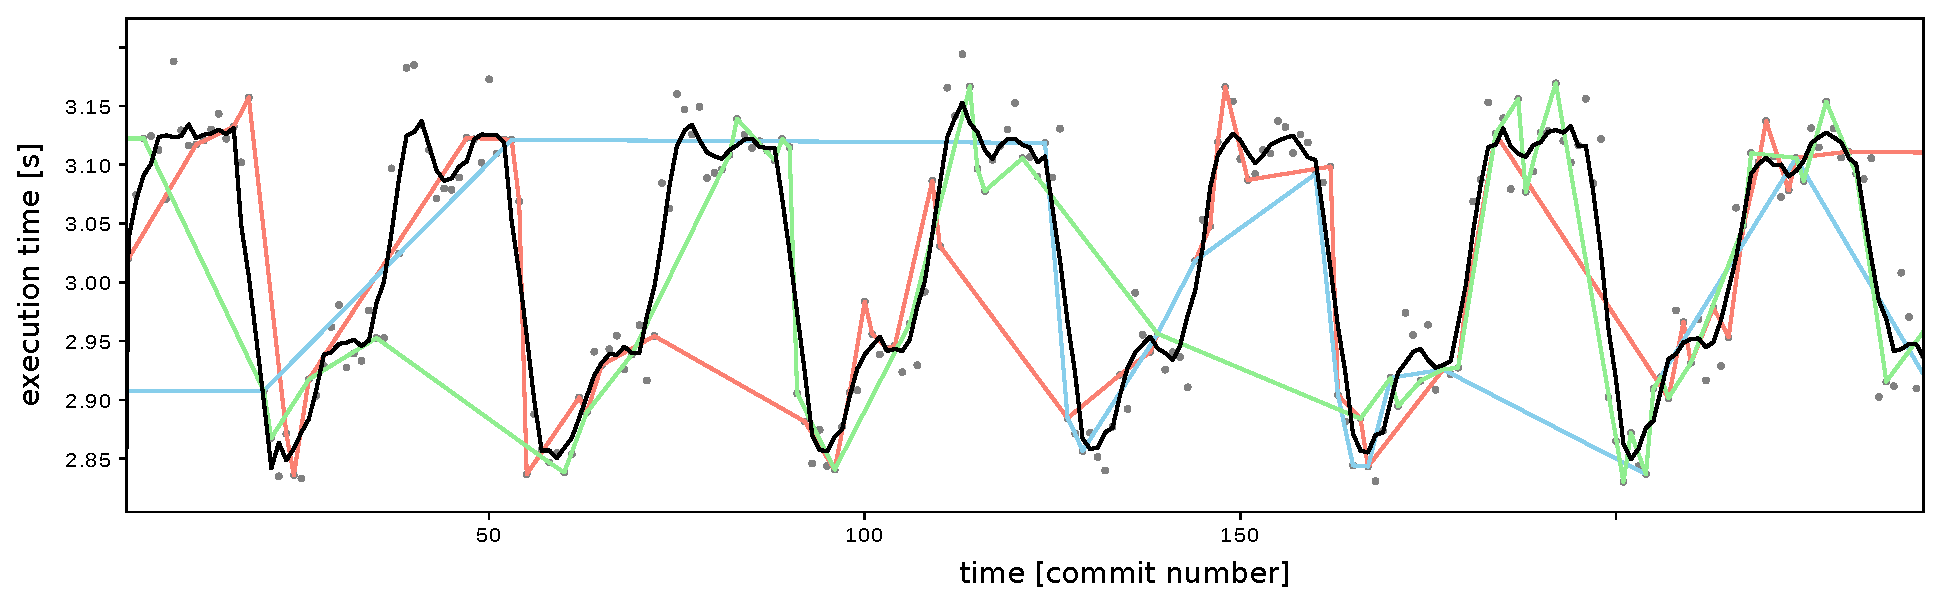
\includegraphics[width=0.95\textwidth]{images/approximations.eps}
	\caption{Performance history approximations with different accuracy results.}
	\label{fig:approximation_accuracy}
\end{figure}

In Figure~\ref{fig:approximation_accuracy}, we illustrate performance history
approximations with different accuracy. The grey scatter plot depicts the
average performance measurements per revision, and the black curve represents
the moving median thereof. The green, blue, and orange curves are respective
approximations. One can see that the green and orange approximation are a more
accurate approximation than the blue one since they more closely follow the
overall performance history.

We evaluated all five revision sampling strategies
for two different configurable software systems. The first system, GNU XZ, is
an open-source file compression tool that is widely used among the open-source
community. It exhibits a number of configurations options via run-time
parameters from which we derived 36 variants using pair-wise sampling. The
second system, x264 is a free implementation of, and encoder for the H.264
video compression standard, commonly known as MP4. Similarly to GNU XZ, it can
be configured using a wide range of run-time parameters from which we derived
eight variants using pair-wise sampling.  A detailed description of the systems’
configuration options and how we derived the feature model is presented in
chapter\,\ref{chapter:6}.

For both systems, we obtained a clone of
their respective git repositories and, as far as possible, compiled each
version: 1,135 for GNU XZ and 2,851 for x264. For GNU XZ, we selected a
standard file compression benchmark, the Canterbury corpus (2.8~MB), for GNU XZ
since it contains different kinds of data (binary as well as plain text). For
x264, we selected an uncompressed movie clip of 79.9~MB as a benchmark. All
performance measurements (execution time) were conducted on a Linux machine
(Debian 8) with a Intel Xeon E5-2680 v2 with 2.8~GHz and 16 GB RAM. For each
version and variant, we repeated the experiment five times and selected the
median of the measurements to exclude extreme measurements.

\subsection{Result Description}
For both assessed systems, we first present the overall performance history to
give an impression of its overall shape. In
Figure~\ref{fig:overall_performance_history}, for both systems, we show the
average performance measurements per revision, calculated as the arithmetic
mean over all 36 and eight variants, respectively.

\begin{figure}[!htb]
\def\tabularxcolumn#1{m{#1}}
\begin{tabularx}{\linewidth}{@{}cXX@{}}
\centering
\begin{tabular}{c}
\subfloat[Average performance history for GNU XZ]
{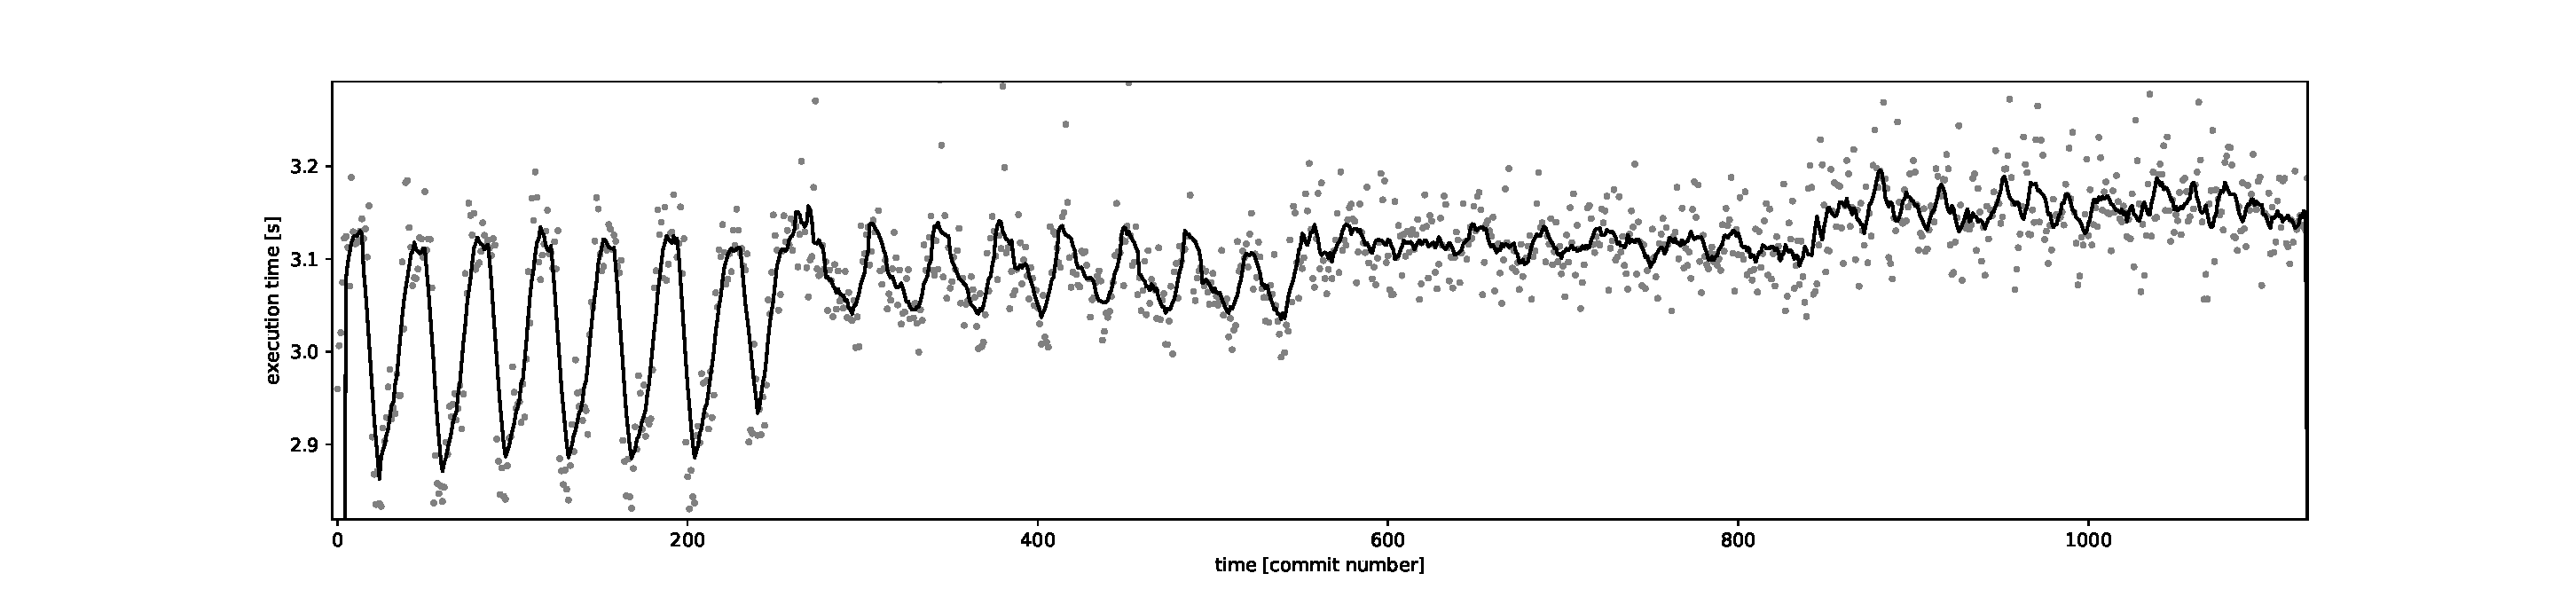
\includegraphics[width=1.0\textwidth]{images/performance_xz.eps}}
\\
\subfloat[Average performance history for x264]
{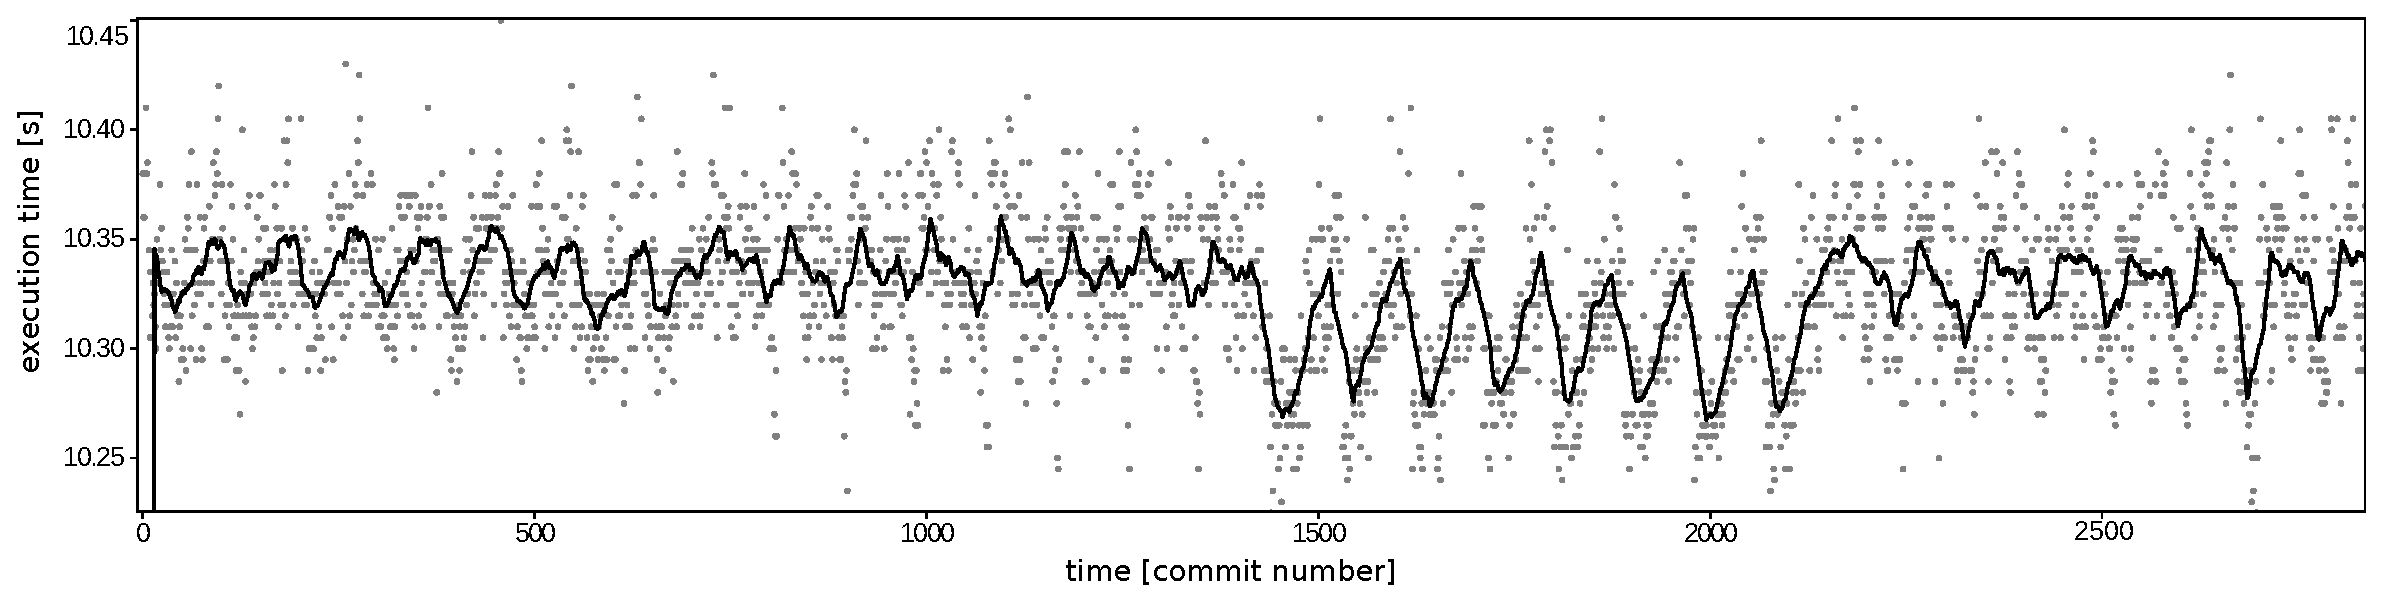
\includegraphics[width=1.0\textwidth]{images/performance_x264.eps}}
\end{tabular}
\end{tabularx}
\caption{Average performance history per version for both GNU XZ and x264}
\label{fig:overall_performance_history}
\end{figure}

For GNU XZ, in the beginning, the performance measurements fluctuate
significantly with an amplitude of up to 0.4 seconds, yet the amplitude
decreases over time. Moreover, the overall trend of the performance
measurements indicates an increase in execution time. This overall trend along
with the decreasing amplitude of fluctuations might indicate a software
architecture that is getting more stable over time, yet becomes slower over
time as well, which is in line with the theory of technical debt mentioned
earlier \citep{guo_tracking_2011}. However, for x264, we could not identify
such an overall trend as the performance measures remain stable for most of the version
history. Only for the time span between commit 1,400 and 2,100, performance
measures fluctuate around a smaller level of execution time. In conclusion,
both systems’ performance histories exhibit local fluctuations, yet the
fluctuation range for x264 remains stable throughout the entire version history
while for GNU XZ, the fluctuation range decreases as the software evolves.
Moreover, for GNU XZ, the frequency of fluctuations, i.e., the number of
fluctuations in a time frame, decreases over time, while it almost remains
stable for x264.

\paragraph{Accuracy Evaluation.} We were able to accurately approximate the
performance history curve for GNU XZ with different revision sampling
strategies. Our first comparison comprises keyword sampling, version
lifetime segmentation, and change size coverage sampling. In addition, we
compared those three sampling strategies to a baseline random sampling
approach, whereby $n$ arbitrary revisions have been selected. While the other
three sampling strategies are deterministic, we repeated the random sampling a
hundred times per revision to minimize variance. For the comparison, we sweeped
the desired sample size for each software system from one to the total number
of commits, respectively.

\begin{figure}[!htb]
\def\tabularxcolumn#1{m{#1}}
\begin{tabularx}{\linewidth}{@{}cXX@{}}
\centering
\begin{tabular}{c}
\subfloat[GNU XZ]
{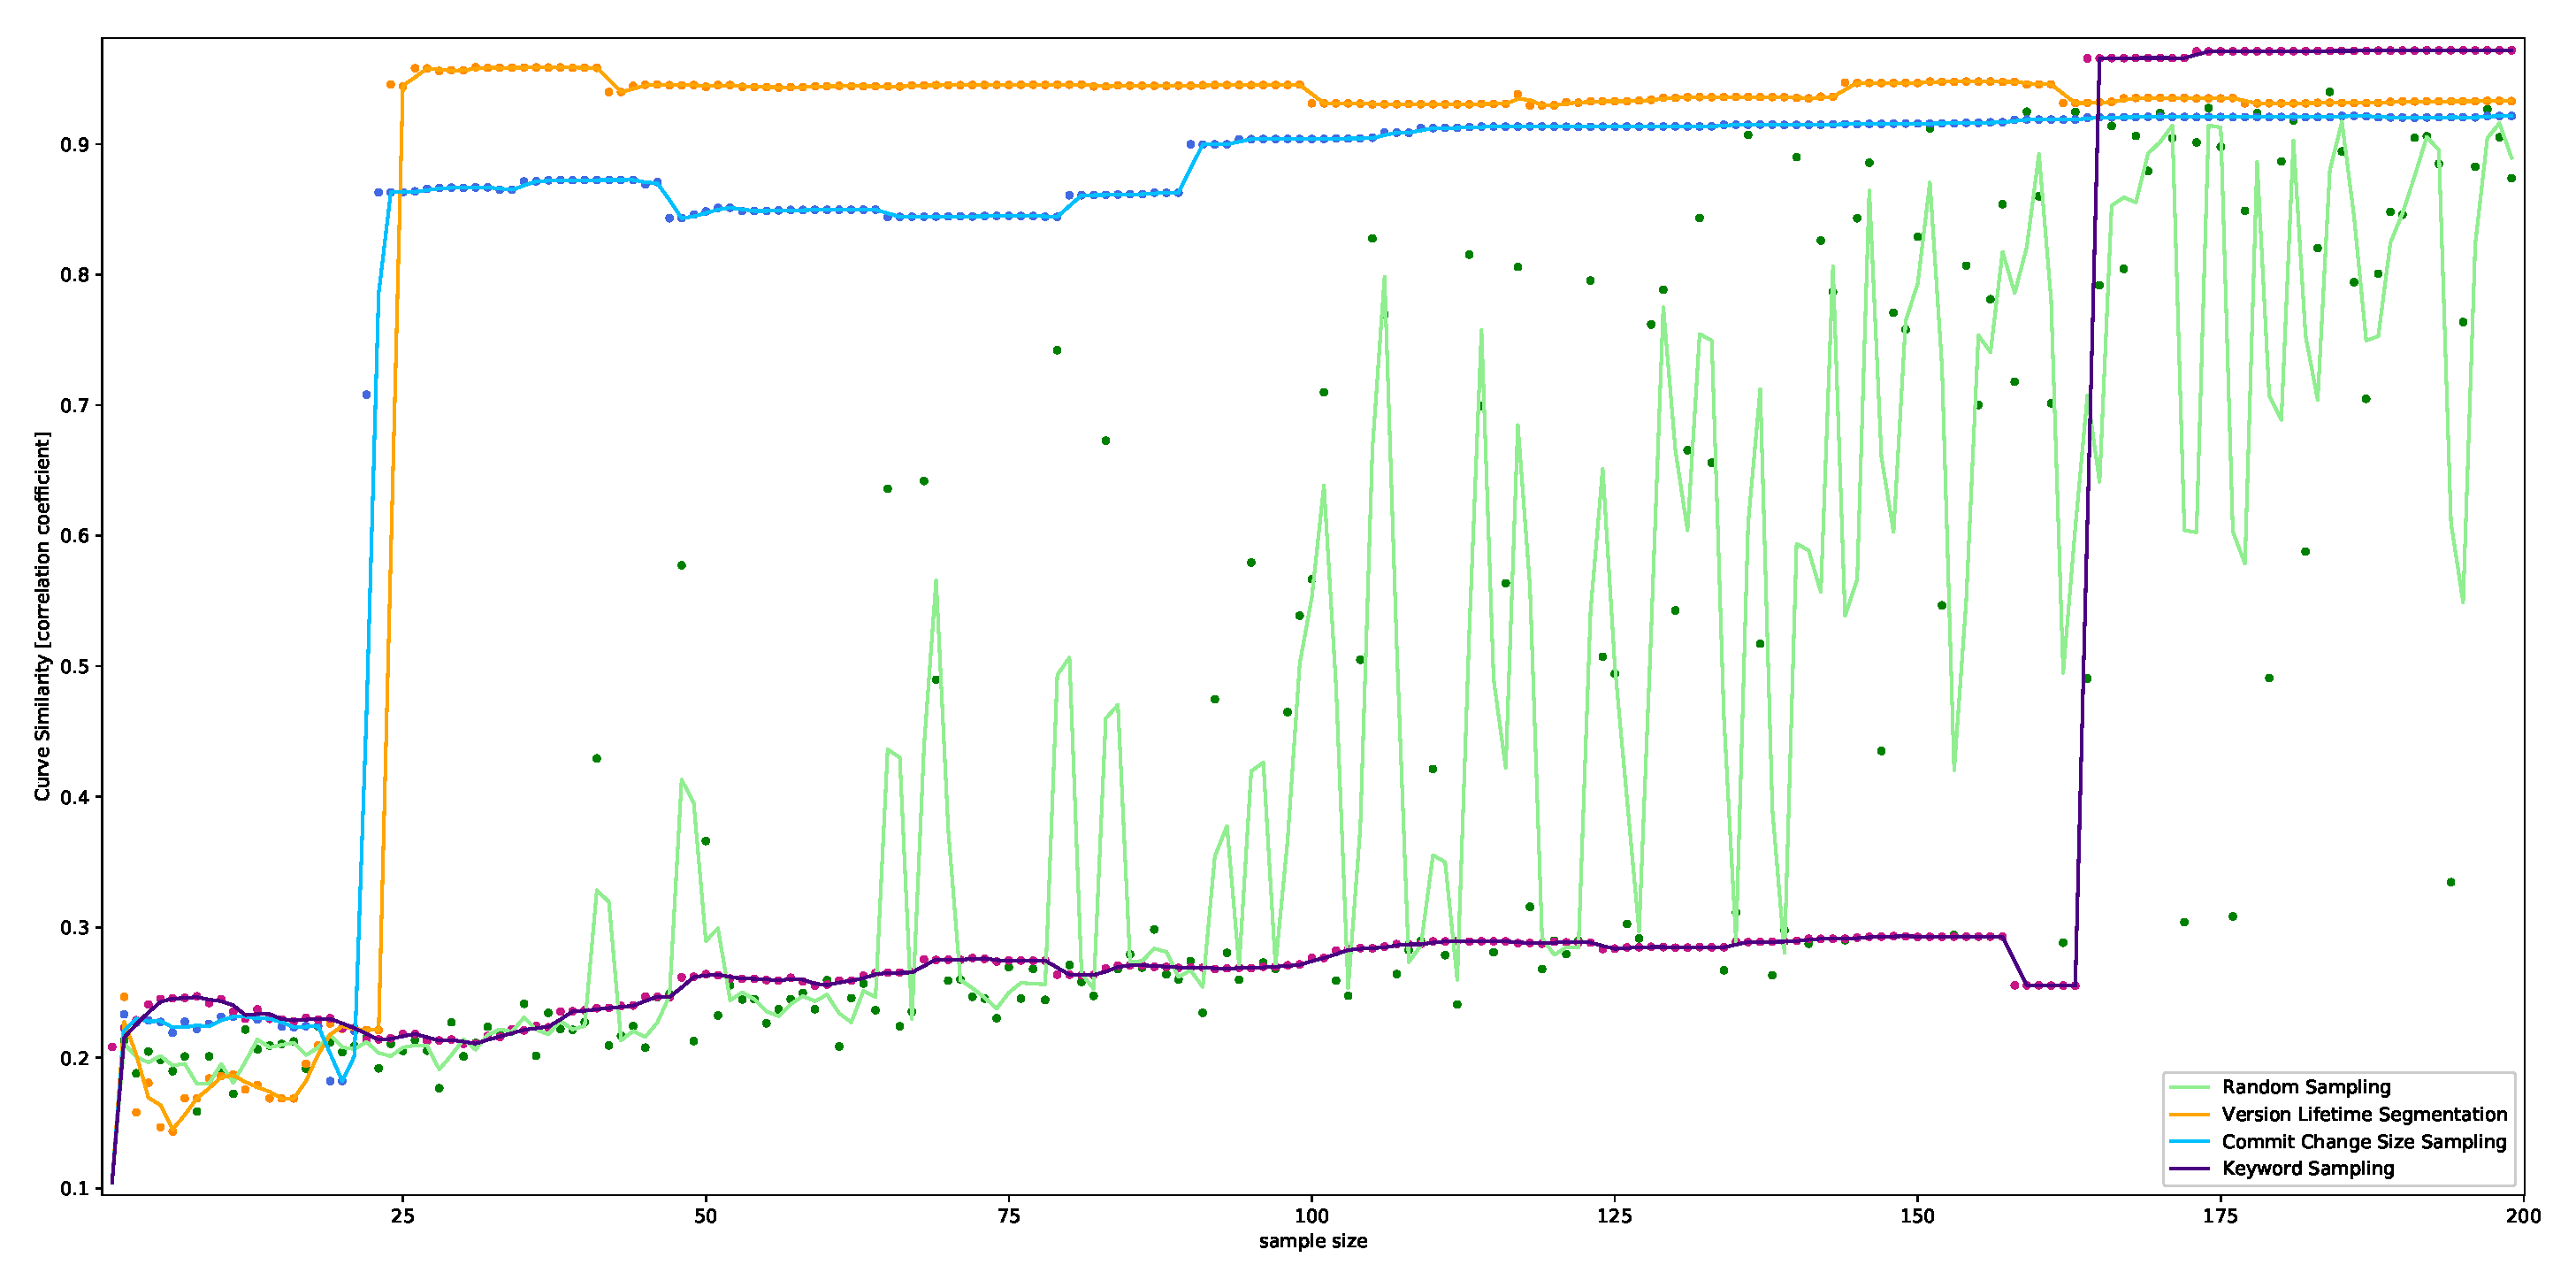
\includegraphics[width=0.99\textwidth]{images/accuracy_xz.eps}}\\
\subfloat[x264]
{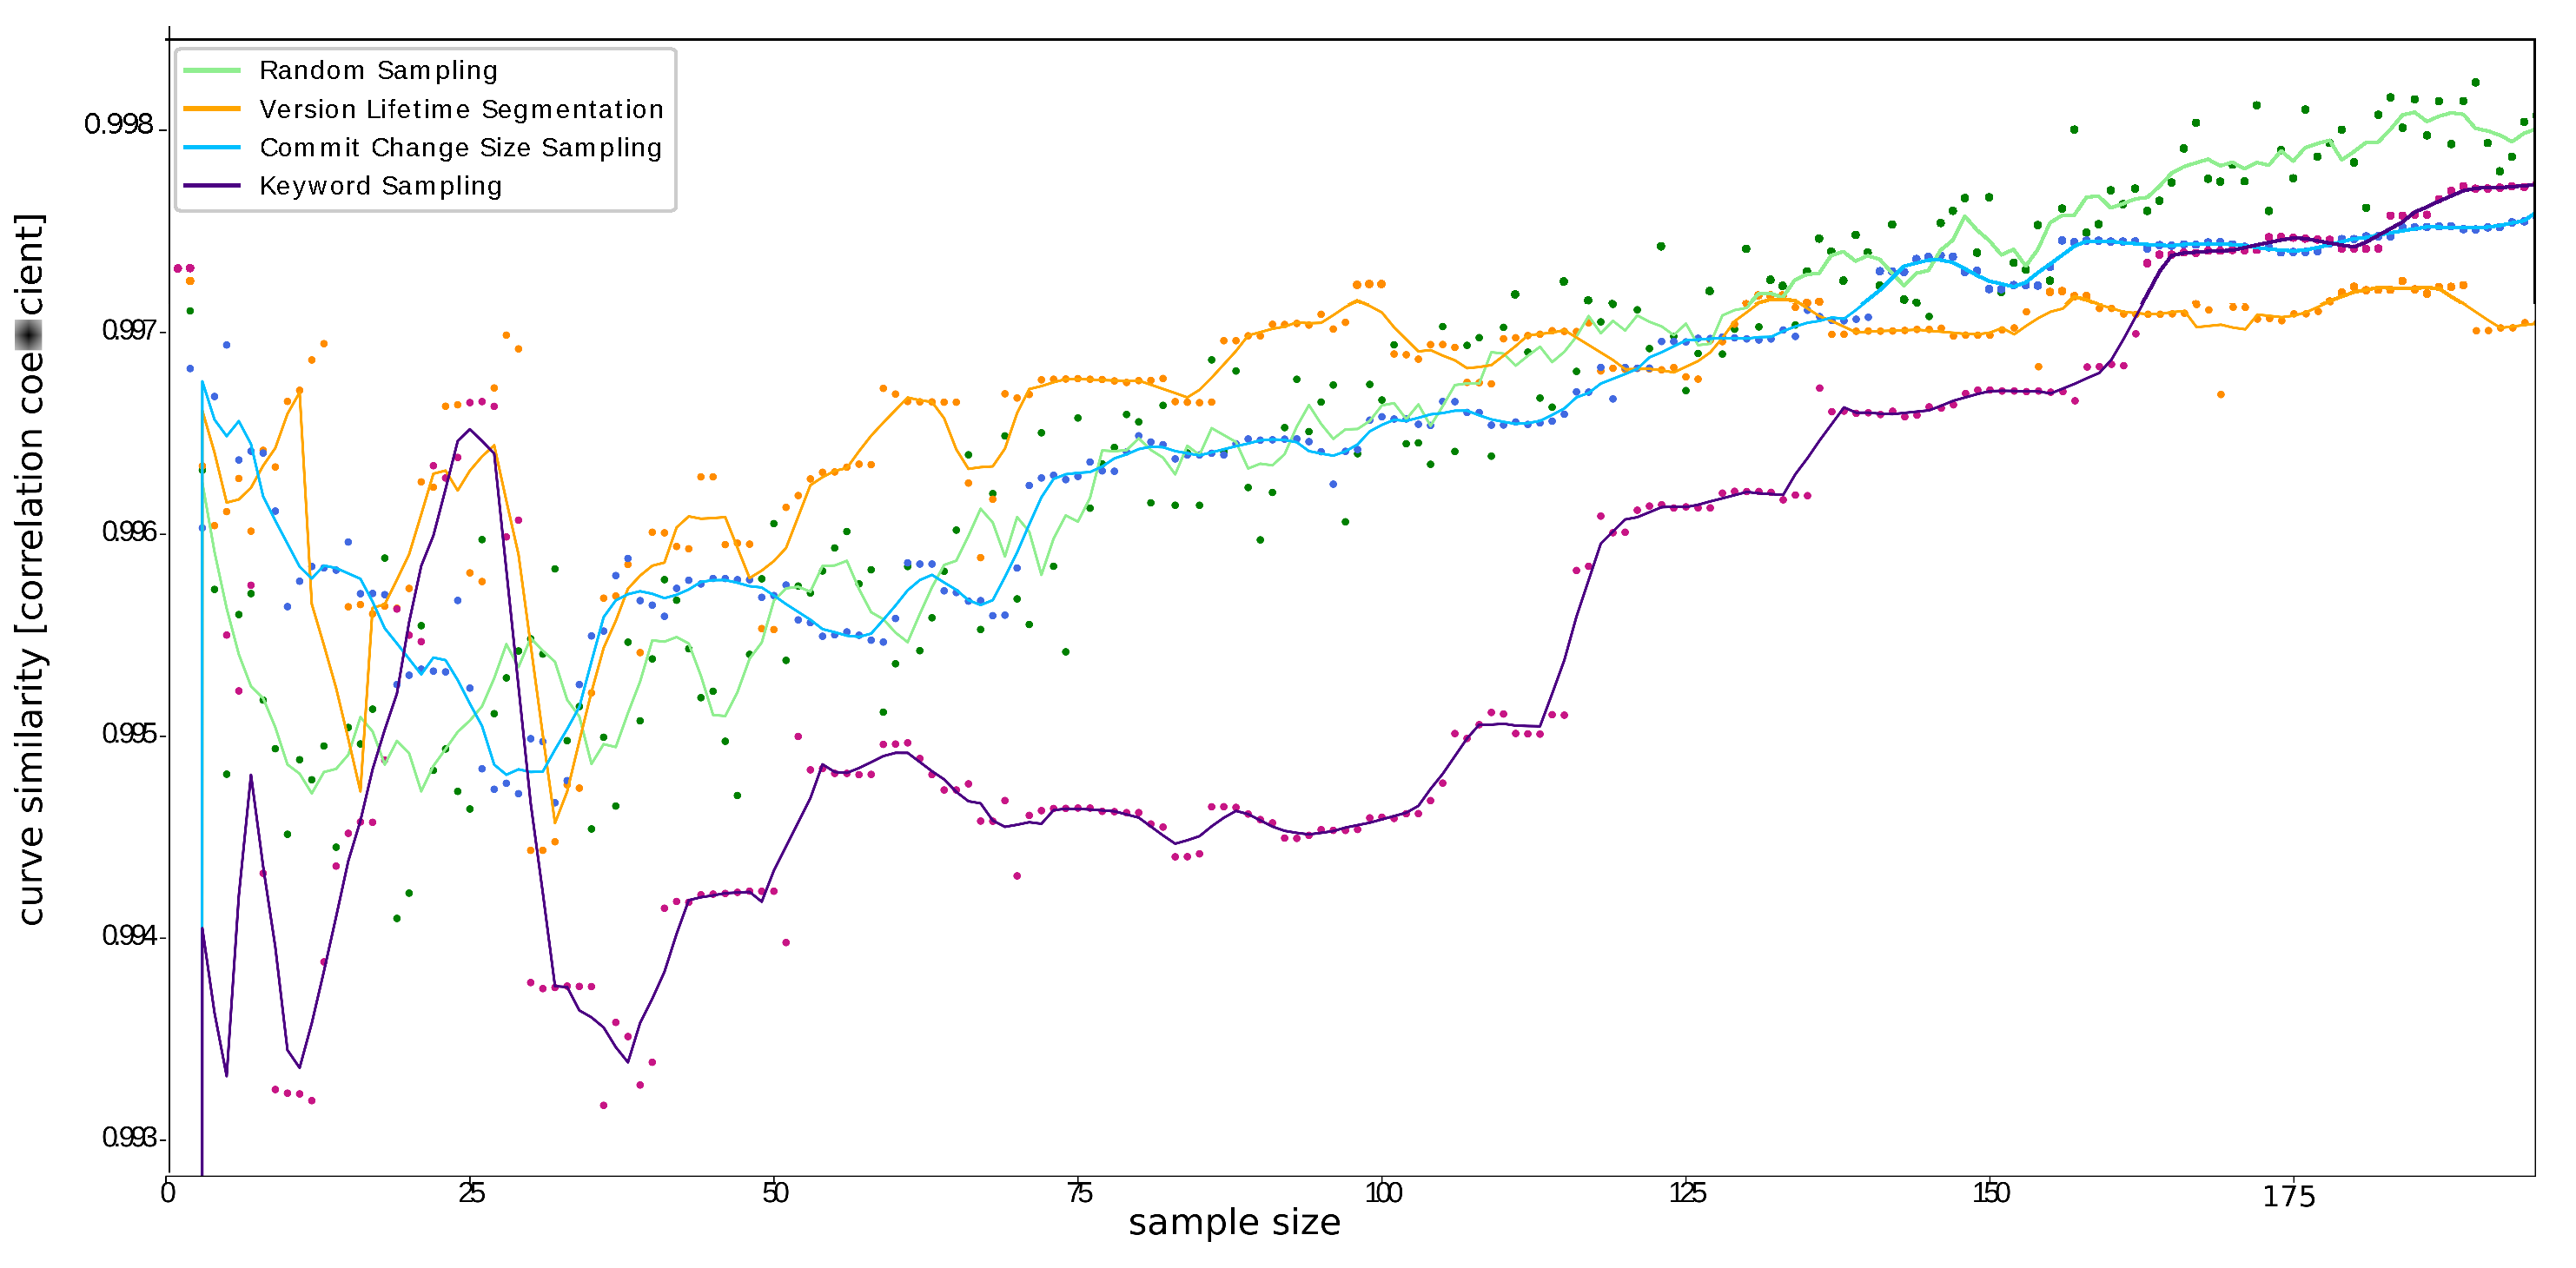
\includegraphics[width=0.99\textwidth]{images/accuracy_x264.eps}}
\end{tabular}
\end{tabularx}
\caption{Accuracy of four different sampling strategies:
version lifetime sampling, random sampling, commit change size sampling, and keyword sampling.}
\label{fig:accuracy_per_strategy}
\end{figure}

In Figure~\ref{fig:accuracy_per_strategy}, we illustrate the accuracy
measurements for four different sampling strategies. For GNU XZ, keyword
sampling and random sampling performed relatively poorly. Compared to version
lifetime sampling and commit change size sampling, they did not achieve an
acceptable level of accuracy. For x264, version lifetime sampling and commit
change size sampling did not perform significantly worse than the respective
others. In general, for x264, we achieved far better accuracy measurements for
all applied sampling strategies as accuracy measurements did not fall below
0.9.

\paragraph{Changed-files Sampling.} For changed-files sampling, we chose a different type of visualization since the
sampling strategy works with two parameters, the initial learning sample size,
and the desired sample size. We visualize the accuracy as a heat map, whereby
combinations of initial learning sample size and desired sample size are
coordinates, and the color at those coordinates represents the corresponding
accuracy measurements. Moreover, we let the sampling strategy operate in two
different modes. First, we selected the initial learning sample randomly, and
second, we selected the change size coverage sampling. We illustrate the
accuracy measurements for both modes in
Figure\,\ref{fig:accuracy_file_sampling1}
and\,\ref{fig:accuracy_file_sampling2}, respectively.

For the experiments with randomly selected initial learning samples in
Figure\,\ref{fig:accuracy_file_sampling1},  for GNU XZ, the accuracy increases
for greater sample sizes.
Moreover, the spread of accuracy decreases for greater training sample sizes. That is,
when learning the relation of changed files and performance changes from a
larger selection of revisions, fewer revisions are required for the actual
sample to achieve a certain accuracy. For the experiments, where the initial
learning samples were selected using the commit change size sampling, as
illustrated in Figure\,\ref{fig:accuracy_file_sampling2}, we see that the
general level of accuracy is significantly higher. For instance, for GNU XZ, the accuracy ranges from 0.6 up
to almost 1.0. In contrast to the previous mode, even a small training sample
of 100 to 200 revisions can be sufficient to achieve reasonable accuracy.
Moreover, for a small sample size, but a great training sample size, the
accuracy degrades.

Following the results for the previous sampling strategies, for x264, we also
achieved high accuracy measurements for both changed-files sampling with random
sampling as well as commit change size sampling. However, we did not measure
any significant influence of either segmentation technique and accuracy did
almost never vary for any combination of parameters.


\begin{figure}[!htb]
\def\tabularxcolumn#1{m{#1}}
\begin{tabularx}{\linewidth}{@{}cXX@{}}
\centering
\begin{tabular}{c}
\subfloat[GNU XZ]
{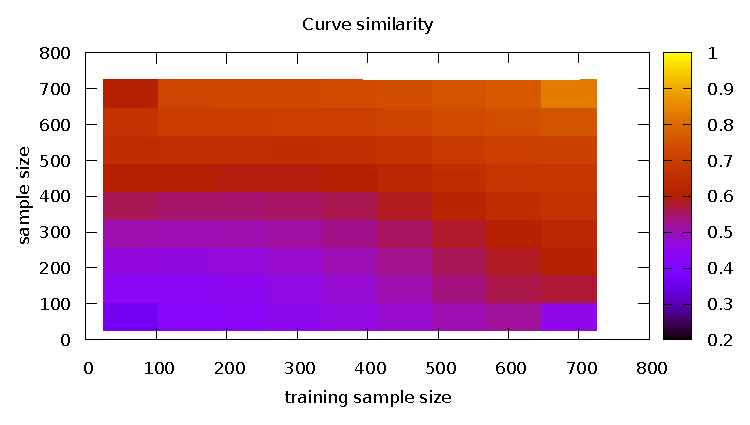
\includegraphics[width=0.95\textwidth]{images/xz_mode0.eps}}\\
\subfloat[x264]
{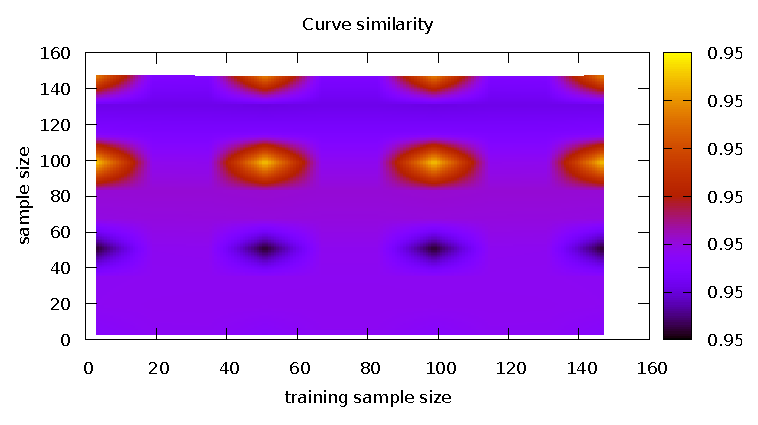
\includegraphics[width=0.95\textwidth]{images/x264_filesampling_0.eps}}
\end{tabular}
\end{tabularx}
\caption{Accuracy of changed-files sampling with randomly selected initial
learning sample for GNU XZ and x264}
\label{fig:accuracy_file_sampling1}
\end{figure}

\begin{figure}[!htb]
\def\tabularxcolumn#1{m{#1}}
\begin{tabularx}{\linewidth}{@{}cXX@{}}
\centering
\begin{tabular}{c}
\subfloat[GNU XZ]
{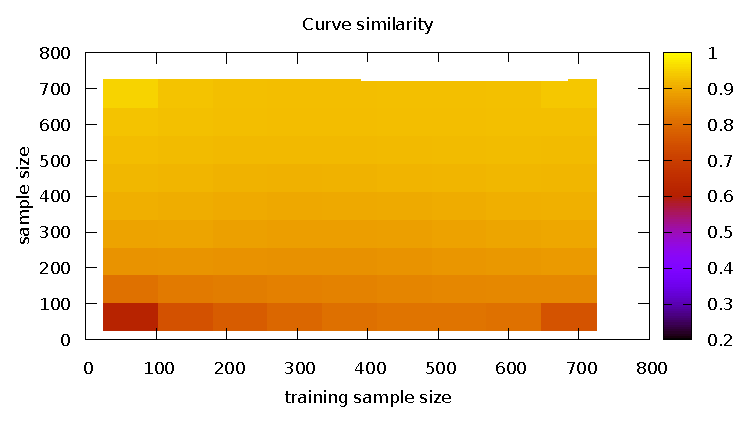
\includegraphics[width=0.95\textwidth]{images/xz_mode1.eps}}\\
\subfloat[x264]
{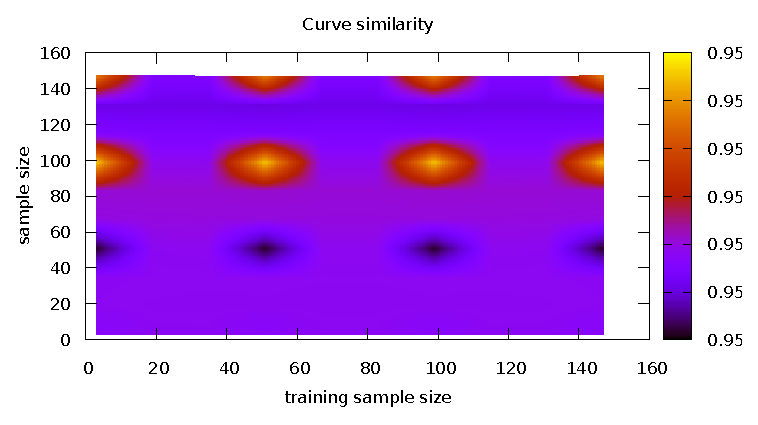
\includegraphics[width=0.95\textwidth]{images/x264_filesampling_1.eps}}
\end{tabular}
\end{tabularx}
\caption{Accuracy of changed-files sampling with the initial
learning sample selected using commit change size sampling; for GNU XZ and
x264}
\label{fig:accuracy_file_sampling2}
\end{figure}

\paragraph{Bisection Sampling.} 
For the last sampling strategy, we continue using the same visualization
technique as for changed-files sampling. Again, this sampling strategy requires
two parameters, an initial sample size $a$, and a number of extension steps $b$
to perform. The initial sample of size $a$ can be selected randomly, or using
version lifetime sampling. In Figures\,\ref{fig:accuracy_bisect1}
and\,\ref{fig:accuracy_bisect2} we illustrate the accuracy measurements for both modes, respectively. We see that for the first operation
mode in Figure\,\ref{fig:accuracy_bisect1} with random sampling, the overall
accuracy is increases with a greater size of the initial sample size, which is in line with our
observations for pure random sampling. The number of extension steps, however,
does not exhibit a significant influence on the accuracy, yet only for a small
initial sample size, where accuracy spread is high. Contrary to the first
operation mode, in Figure\,\ref{fig:accuracy_bisect2}, we illustrate the
accuracy measurements for the second operation mode, where the initial sample is obtained via version
lifetime segmentation. While most of the description of the previous operation
mode also applies to this one, the operation mode in general performs better, as the
minimum accuracy measurement is about 0.9.

Similar to the accuracy measurements for changed-files sampling for x264, we
achieve high accuracy measurements for bisection sampling for both combinations
with random sampling as well as version lifetime segmentation, whereby the
latter combination performed slightly better. However, the range of spread for
accuracy measures for both operation modes is negligibly small.

\begin{figure}[t!]
\def\tabularxcolumn#1{m{#1}}
\begin{tabularx}{\linewidth}{@{}cXX@{}}
\centering
\begin{tabular}{c}
\subfloat[GNU XZ]
{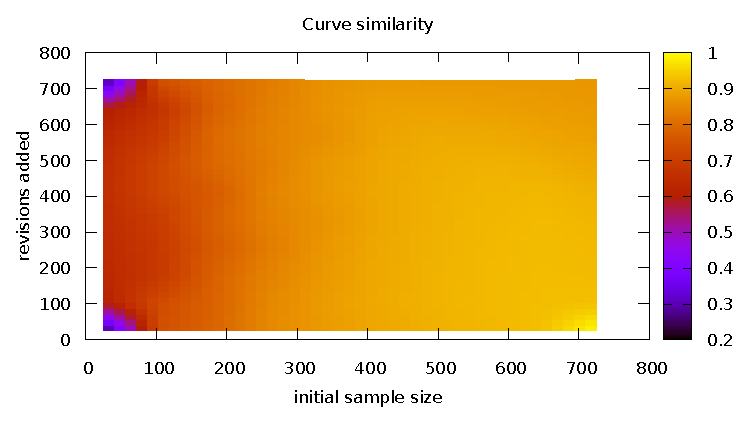
\includegraphics[width=0.95\textwidth]{images/xz_bisect_mode0.eps}}\\
\subfloat[x264]
{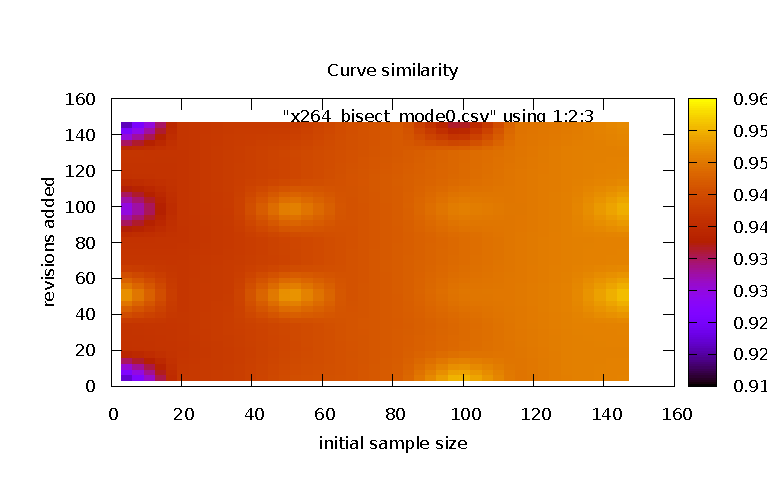
\includegraphics[width=0.95\textwidth]{images/x264_bisection_0.eps}}
\end{tabular}
\end{tabularx}
\caption{Accuracy of bisection sampling with randomly selected initial samples
for GNU XZ and x264}
\label{fig:accuracy_bisect1}
\end{figure}
% bener

%\blindtext

\begin{figure}[t!]
\def\tabularxcolumn#1{m{#1}}
\begin{tabularx}{\linewidth}{@{}cXX@{}}
\centering
\begin{tabular}{c}
\subfloat[GNU XZ]
{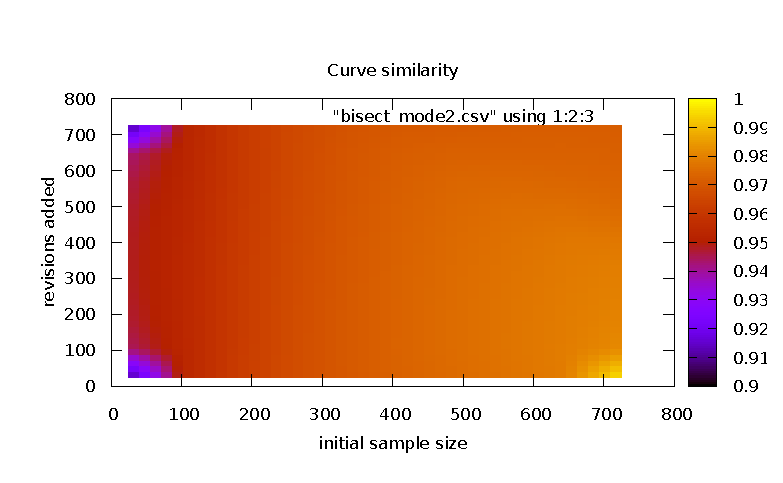
\includegraphics[width=0.85\textwidth]{images/xz_bisect_mode2.eps}}\\
\subfloat[x264]
{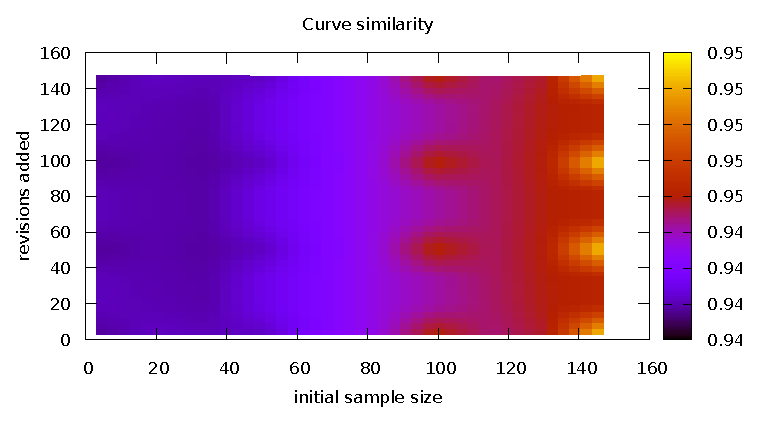
\includegraphics[width=0.85\textwidth]{images/x264_bisection_2.eps}}
\end{tabular}
\end{tabularx}
\caption{Accuracy of bisection sampling with initial samples selected via
version lifetime segmentation for GNU XZ and x264}
\label{fig:accuracy_bisect2}
\end{figure}

\paragraph{Discussion.} The accuracy measurements of the five sampling
strategies presented above differ significantly between the two systems
studied. While the results for GNU XZ are heterogeneous enough to suggest a
sampling strategy over the others, for x264, following the results, every
sampling strategy tested performed well. Furthermore, all accuracy measurements
for x264 seem to remain almost stable for most combinations of input
parameters. That is, to understand the discrepancy between both two systems, we
re-evaluated our definition of accuracy. All accuracy measurements were
calculated as the correlation coefficient between the average performance of
all variants assessed and the interpolation obtained from a subset of the
average performance history. Moreover, for the overall average performance, we
consider a moving mean in order to smooth the performance history curve and
sketch mid- to long-term performance evolution trends. While we obtained
accuracy results of plausible shape for GNU XZ, for x264, the previously described accuracy
measurements appear unlikely.

\begin{figure}[t!]
\centering
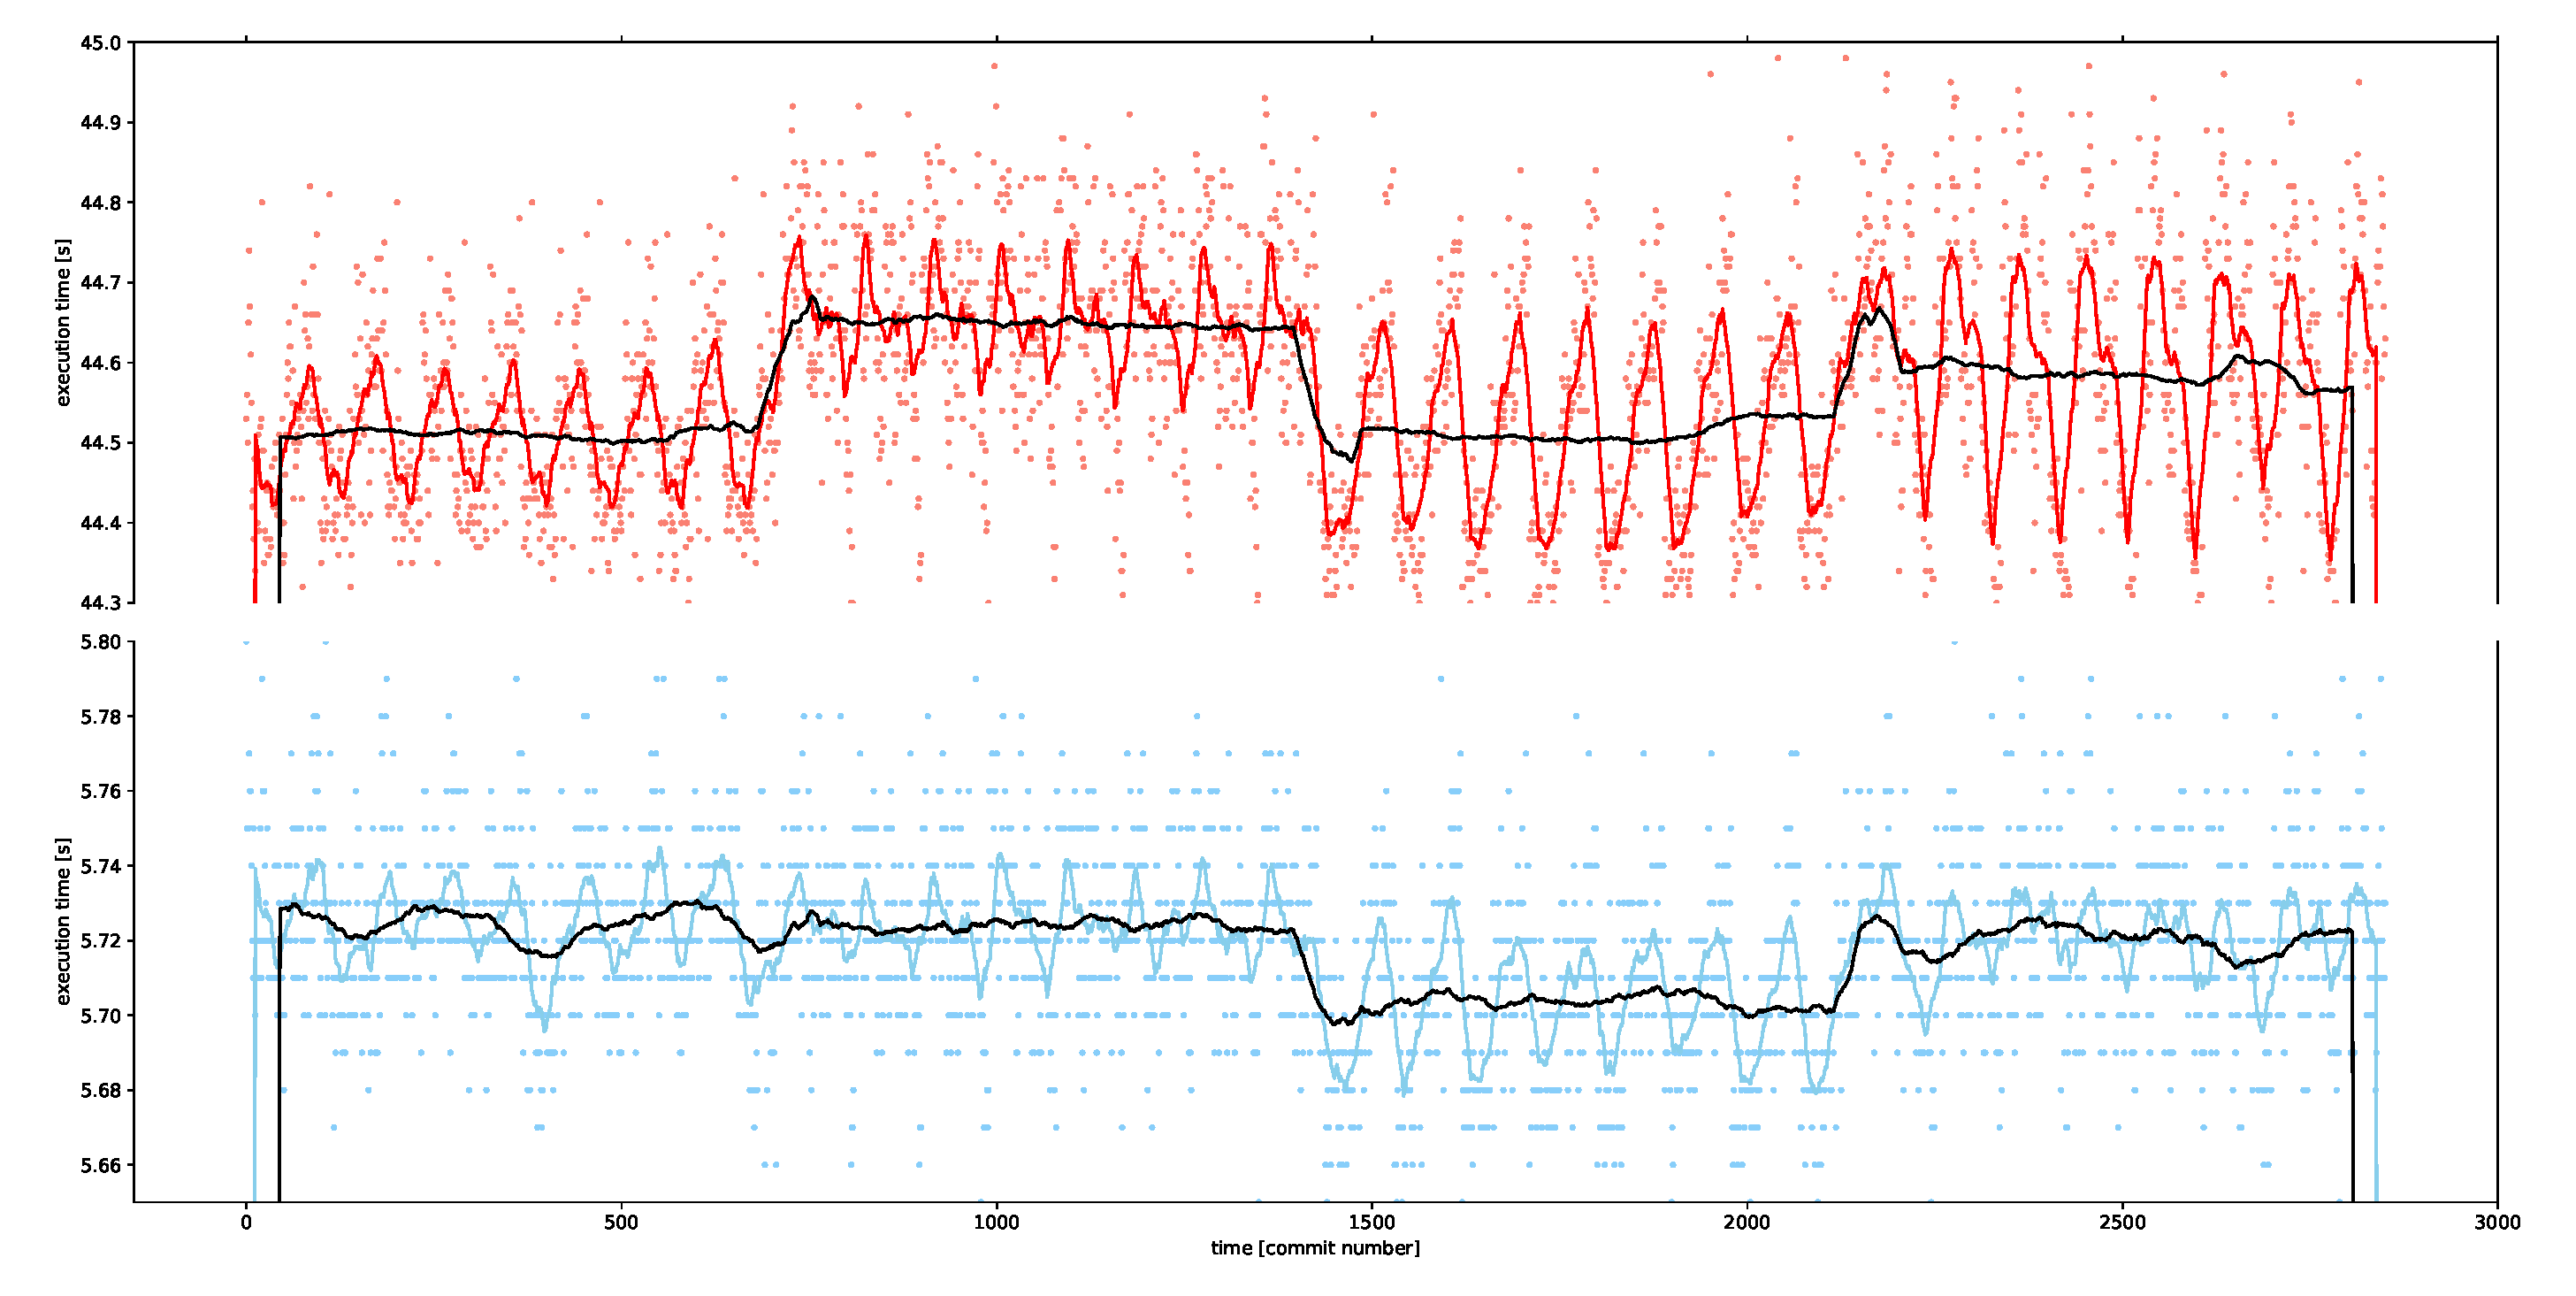
\includegraphics[width=0.99\textwidth]{images/x264_best_worst.eps}
\caption{Performance history for x264: worst-performing variant (top) and
best-performing variant (bottom)}
\label{fig:x264_worstbest}
\end{figure}

We identified two possible causes for those results. First, the smoothing
factor, i.e., the frame size for the moving mean, influences how similar the
smoothed curve looks to a straight line. If a greater smoothing factor is
selected, the performance history curve can easily be approximated with an
interpolation of only two points. Second, the performance history itself can be
shaped quasi-linear. For the latter case, either the performance remains stable
while the software system evolves, or the average performance history does not
exhibit existing performance changes, for instance, when performance changes
only affect few variants, or performance only fluctuates within a small range.
From comparing the average performance history (cf.
Figure~\ref{fig:overall_performance_history}) and the best- and
worst-performing variant (see Figure~\ref{fig:x264_worstbest}) for x264, we
learn that at around commit 650 performance significantly increases for the
best-performing variant, while almost no effect is visible for the
best-performing one as well as for the average performance history. Moreover, the spread range for performance measurements was not more than 0.1 seconds for
the best-performing variant, and 0.15 seconds for the average performance
history. Considering the range of 0.4 to 0.5 seconds for the worst-performing
variant, the differently shaped performance curves suggest that the used
evaluation technique is not necessary suitable to evaluate performance history,
if effects are of too small magnitude or effect range.

\section{Methodological Remarks}\label{sec:revsampling_method}
In the last subsection we have presented the evaluation results for our
revision sampling strategies proposed earlier. Despite different accuracy
measurements, we now put the strategies and their cost-efficiency in the context
of our methodology. While a high accuracy is desirable, the revision sampling
strategies proposed differ in the required number of performance measurements
For instance, keyword sampling as well as version lifetime segmentation and
commit change size sampling require no revision to be assessed at all, while
for changed-files sampling and bisection sampling the number of revisions that
are necessary to assess exceeds the resulting sample size. In
Table~\ref{tab:revsampling_overview} we present an overview of the five proposed sampling strategies along with their
parameter description, number of required performance measurements, i.e.,
revisions to assess, and the resulting sample size depending on the strategies
parameters.

With respect to accuracy, from the evaluation we have learned that commit
change size sampling, version lifetime segmentation, changed-files sampling with
commit change size sampling, and bisection sampling with version lifetime segmentation performed best.
Commit change size sampling does not require any performance measurements. We
consider the cost of collecting information about all commits as well as
ordering them with respect to commit change or lifetime coverage as constant
since the time required only depends on the host machine used for sampling, and it only
required a few seconds for our evaluation setup. 

\begin{table}[t!]
\centering
\begin{tabular}{C{3cm}L{5cm}L{3cm}L{3cm}}
\toprule
 \textbf{Sampling Strategy} & \textbf{Parameters} & \textbf{Required
 measurements} & \textbf{Resulting sample size} \\
 \midrule
 Keyword Sampling & Sample Size $N$ & $0$ & $N$\\
 \midrule 
 Version Lifetime Segmentation & Sample Size $N$ & $0$ & $N$\\
 \midrule 
  Commit Change Size Sampling & Sample Size $N$ & $0$ & $N$\\
 \midrule 
  Changed-files Sampling & {Sample Size $N$\linebreak Learning Sample Size $M$}
  & $2\times M$ & $M + N$
  \\
 \midrule 
  Bisection Sampling & {Sample Size $N$\linebreak Initial Sample Size $M$} &
  $2\times M$ & $M + N$
  \\
 \bottomrule
\end{tabular}
\caption{Overview of different sampling strategies, required parameters,
performance measurements, and resulting sample sizes}
\label{tab:revsampling_overview}
\end{table}

Next, changed-files sampling with commit change size sampling has shown
acceptable accuracy, yet only for relatively great sample sizes compared to
pure commit change size sampling. Moreover, the selection of a suitable
learning sample size does not seem trivial, as accuracy increased up to a
certain learning sample size, yet decreased for greater sample sizes. That is,
it is hard to estimate a sweet spot size for a learning sample that on the one
hand contains enough knowledge to learn a possible relation between files
changed an performance changes on the one hand, and on the other hand does not
contain too many revisions diluting the learning sample's informative value. 

Finally, bisection sampling with version lifetime segmentation has shown high
accuracy for almost all parameter combinations, yet compared to the previous
sampling strategies, the required number of revisions to assess is
significantly higher. Contrary to changed-files sampling that also utilizes an
initial sample for which twice the number of measurements is required, this
sampling strategy additionally requires two performance requirements for each
segmentation step.\\

In conclusion, based on our case study we advocate the use of commit change
size version lifetime segmentation sampling as the ratio of required performance
measurements and resulting accuracy is optimal. However, note that the case study corpus only contains two
software systems and that our results are far from being representative.
However, based on our observations, we were not able to disprove the assumption
of a relation between a commit’s change size and its potential influence on performance.
